\documentclass[12pt,twoside]{article}

\usepackage[T1]{fontenc}
\usepackage[utf8]{inputenc}
\usepackage[spanish]{babel}

\let\layoutspanish\relax
\addto\captionsspanish{\def\tablename{Tabla}}
\unaccentedoperators

\usepackage[a4paper]{geometry}
  \geometry{hmargin={2.5cm,2.5cm},height=22cm}
  
\renewcommand{\baselinestretch}{1.2}  
\setlength{\partopsep}{0pt}
\setlength{\itemsep}{0pt}
\setlength{\topsep}{0pt}
\setlength{\parsep}{0pt}
\setlength{\parskip}{0.25\baselineskip}

\renewcommand{\textfraction}{0.1}
\renewcommand{\topfraction}{1}
\renewcommand{\bottomfraction}{1}
\renewcommand{\floatpagefraction}{1}

\setcounter{totalnumber}{5}
\setcounter{topnumber}{3}
\setcounter{bottomnumber}{2}

\usepackage{caption}


\usepackage{indentfirst}

\usepackage[pdftex]{color}
\usepackage[table,xcdraw]{xcolor}
\usepackage{float}
\usepackage{tabularx}

\usepackage[pdftex]{graphicx}
\usepackage{amsmath}
\allowdisplaybreaks 
\usepackage{amssymb}
\usepackage{amsfonts} 
\usepackage{enumerate}

\usepackage{fancyhdr}

\newcommand{\RunningAuthor}{Ginés Meca Carbonell}
\newcommand{\Author}[1]{\renewcommand{\RunningAuthor}{#1}}
\renewcommand{\leftmark}{\RunningAuthor}

\newcommand{\RunningTitle}{Métodos de Machine Learning basados en Árboles de Decisión.}
\newcommand{\Title}[1]{\renewcommand{\RunningTitle}{#1}}
\renewcommand{\rightmark}{\RunningTitle}

\pagestyle{fancy}
\fancyhf{}
\fancyhead[LO]{\small \slshape \leftmark}    
\fancyhead[RE]{\small \slshape \rightmark}   
\fancyhead[RO,LE]{\small \slshape \thepage}  

\renewcommand{\headrulewidth}{0.6pt}         
\renewcommand{\footrulewidth}{0pt}           
                                             
\setlength{\headheight}{1.5\headheight}      

\fancypagestyle{plain}{%                     
  \fancyhf{}                                 
  \setlength{\headwidth}{\textwidth}
  \fancyfoot[C]{\small \slshape \thepage}    
  \renewcommand{\headrulewidth}{0pt}
  \renewcommand{\footrulewidth}{0pt}
  }
  
\newcommand{\abs}[1]{\ensuremath{|#1|}}
\usepackage{rotating}

\usepackage{hyperref}

\title{Métodos de Machine Learning basados en Árboles de Decisión}
\author{Ginés Meca Carbonell\\*[1em]
\begin{minipage}{0.75\textwidth}
\footnotesize \itshape
\begin{center}
Universidad de Alicante \\
4º de Grado en Matemáticas
\end{center}
\end{minipage}
}
\date{Julio 2022}

\usepackage{pdfpages}




\begin{document}


\includepdf[pages=1]{anexo-1-portada-memoria-tfg-matematicas.pdf}



\section*{Resumen}

\emph{En este trabajo, se ha estudiado el conjunto de algoritmos de Machine Learning que derivan de los árboles de decisión, confeccionando un mapa conceptual de modelos de manera que sea posible clasificarlos en cuanto a aspectos teóricos y reconocer sus principales características. Los árboles de decisión son algoritmos capaces de aprender de variables explicativas de datos conocidos y realizar predicciones sobre datos nuevos. Mediante diferentes tipos de combinaciones, se llegan a dos grandes familias de modelos más complejos: algoritmos de bagging y algoritmos de boosting. Estos modelos de mayor complejidad son capaces de conseguir un significativo aumento de precisión, especialmente cuando se enfrentan a grandes cantidades de datos. Por ello, son muy utilizados e imprescindibles actualmente para trabajar en Big Data.}

\emph{Para poder profundizar y realizar un correcto análisis de los modelos más complejos, en la primera parte se ha estudiado el proceso de construcción de árboles de decisión. En particular, se ha analizado el algoritmo CART, que es el más utilizado. A lo largo de esta sección, se introducen diferentes nociones como los criterios de escisión, los criterios de parada o la asignación de valores de respuesta.}

\emph{En la segunda parte del trabajo, se han estudiado los algoritmos de bagging y boosting por separado. Respecto a los algoritmos de bagging, se han explicado las ideas principales de su funcionamiento. En cuanto a los algoritmos de boosting, se ha realizado un detallado análisis de cada uno de ellos, explicando cuáles son las funciones y parámetros implicados así como el proceso exacto que aplican para conseguir disminuir el error de predicción.}

\emph{Por último, tras la explicación de cada tipo de algoritmo, se ha realizado un ejemplo práctico a fin de ilustrar aquello explicado de manera teórica. También, se han utilizado estos ejemplos para realizar una comparación en términos de precisión y tiempo computacional de todos los modelos explicados, señalando diferencias entre ellos y comprobando que se cumplen ciertas características previamente explicadas. El código utilizado ha sido elaborado en exclusiva para el trabajo y se encuentra en el repositorio de GitHub del autor.}

\textbf{Palabras clave:} CART, Bagging, Boosting, Machine Learning



\newpage



\section*{Abstract}

\emph{In this research, it has been studied the set of Machine Learning algorithms derived from decision trees, making a conceptual map of models so that we can classify it according to their theoretical aspects and we can recognize their main features. Decision trees are algorithms capable of learning from known data explanatory variables and making predictions about new data. Through different types of combinations, we obtain two families of more complex models: bagging algorithms and boosting algorithms. These models are able to increase significatively the accuracy, specially when they have to deal with large amounts of data. That's why they are very useful models and they have become essential in Big Data technologies.}

\emph{In order to study in more detail and analyze correctly the complex models introduced, in the first part of this work it has studied the decision trees building process. In particular, it has been analyzed the most popular algorithm: CART. Along this section, different notions like split criterions, stop criterions or output assignment are introduced.}

\emph{In the second part of this work, it has studied bagging and boosting algorithms by separate. In regard to bagging algorithms, it has been explained the main ideas related to their functioning. Referring to boosting algorithms, it has been done a complete analysis of each of them, explaining which are the functions and parameters implied as well as the exact process applied to reduce the prediction error.}

\emph{Finally, after each type of algorithms explanation, solve a practical example has been solved in order to illustrate what the theory explained. Furthermore, these examples have been used to make a accuracy and running time comparison of all models, showing the differences between them and checking the features explained previously. The code used has been developed exclusively for the research and it's available in the author's GitHub repository.}

\textbf{Key words:} CART, Bagging, Boosting, Machine Learning



\newpage



\tableofcontents



\newpage



\section{Introducción}

En plena era de la información, cada segundo millones de datos viajan entre diferentes lugares del planeta y se guardan formando enormes conjuntos de datos. Además, cada vez hay más instrumentos capaces de recoger información. Donde antes se necesitaba hacer uso de encuestas, ahora existen dispositivos, como los teléfonos móviles, capaces de escribir texto, recoger audio y realizar fotografías y vídeos. Así, la información al alcance es infinita. Es posible conocer cuáles son los conceptos que son tendencia en los buscadores de internet, o cuáles son aquellos audiovisuales que más éxito están teniendo en las redes sociales. Del mismo modo, se  puede acceder al historial de imágenes de la cámara de seguridad de una vivienda o a la tabla que recoge las últimas operaciones de la empresa familiar. Es fácil obtener grandes cantidades de datos de aquello en lo que se está interesado.

Dado que el número de datos manipulados cada vez es mayor, las técnicas utilizadas para analizarlos van evolucionando constantemente. Muchas de las técnicas clásicas del análisis de datos han quedado obsoletas, otras se utilizan para crear algoritmos más complejos. Uno de los algoritmos más conocidos es el de los árboles de decisión. Fueron introducidos por primera vez en 1963 \cite{MO01}, quienes obtuvieron un método muy eficaz a través de un algoritmo muy básico. Actualmente, existen diferentes algoritmos que se pueden emplear a la hora de generar un árbol de decisión: CHAID, C4.5, FACT, QUEST, CRUISE... No obstante, el más conocido, y el que se estudiará en este trabajo, es el algoritmo CART (Classification And Regression Trees), publicado en 1984 \cite{BR03} por Leo Breiman, entre otros. De hecho, fue el propio Breiman quien, haciendo uso de CART, desarrolló años más tarde algoritmos como Bagging \cite{BR01} y Random Forest \cite{BR02}. Paralelamente, la publicación de Freund y Schapire en 1997 \cite{FR01} de un nuevo método basado en boosting daría lugar a otra serie de algoritmos, donde aparecen algoritmos más complejos, como XGBoost, que ocuparán gran parte del trabajo.

Este TFG se centra en analizar a fondo los algoritmos más complejos y novedosos de árboles de decisión. Para ello, se comenzará repasando, brevementeme, el proceso de construcción de los árboles. Después, se dedicará la mayor parte del trabajo a desarrollar los algoritmos derivados de éstos, explicando brevemente los algoritmos de bagging y analizando en profundidad los de boosting, pues emplean técnicas más dificultosas. Para ilustrar los procesos descritos en el trabajo, se han desarrollado diferentes ejemplos. El código empleado para estos ejemplos y para los gráficos y tablas que aparecen a lo largo de la memoria ha sido desarrollado por el autor y se encuentra disponible en GitHub (\url{https://github.com/GinesMeca/TFG}); más detalles en el Anexo (\ref{Anexo}). Por otro lado, se ha utilizado el mismo conjunto de datos a lo largo del proyecto, que se describen a continuación.



\subsection{Datos: Llueve en Australia} \label{sec: subsec11}

El conjunto de datos ``Rain in Australia'' es un dataset formado por mediciones de 20 variables meteorológicas así como la fecha y localidad correspondientes y la información relativa a si llovió o no el día de la medición y el día siguiente, que hacen un total de 23 variables. Se trata de un conjunto de datos público disponible en Kaggle (\url{https://www.kaggle.com/datasets/jsphyg/weather-dataset-rattle-package}). El objetivo será evaluar la capacidad de predicción de lluvia de días futuros de los diferentes algoritmos descritos.

Se dispone de las mediciones de 145.460 días. En la Tabla \ref{tab:01} se muestran los valores de las 23 variables para los 5 primeros casos.
\begin{table}[h]
	\centering
	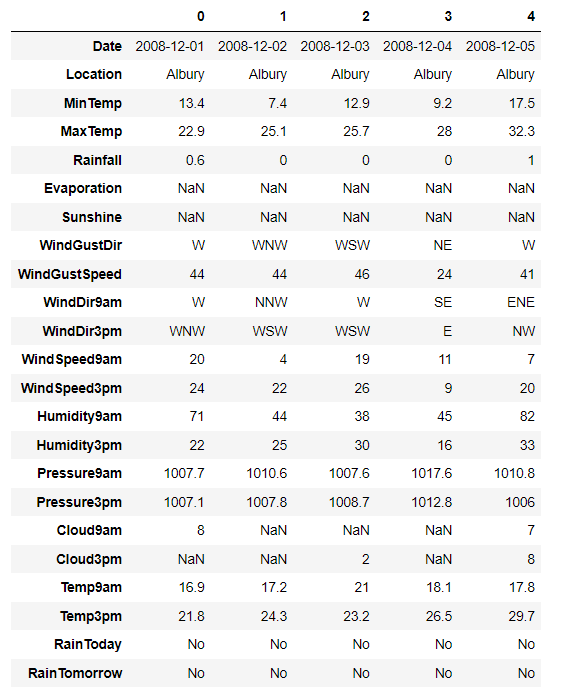
\includegraphics[width = 0.4\textwidth]{Intro_01}
	\caption{Encabezado del dataset donde se muestran las variables en filas y los 5 primeros casos en columnas.}
	\label{tab:01}
\end{table}

En los diferentes ejemplos, se tratará de realizar predicciones de la variable ``Rain Tomorrow''.


\subsection{Evaluación de modelos} \label{subsec:Metodología}

Hoy en día es habitual evaluar un modelo predictivo mediante el método de validación cruzada, proceso que evalúa el error o bien la calidad de un modelo con casos que no han participado en su obtención. A partir de un conjunto de datos, se siguen los siguientes pasos:

\begin{enumerate}
\item Se separa, al azar, el conjunto de datos inicial en dos: datos de entrenamiento y datos de testeo.
\item Se estima el modelo con los datos de entrenamiento.
\item Se aplica el modelo entrenado a los datos de testeo.
\item Se evalúa la precisión de las predicciones realizadas.
\end{enumerate}

Habitualmente, la división del conjunto inicial que da lugar a los subconjuntos de entrenamiento y testeo se realiza de manera aleatoria. No obstante, dado que los datos podrían interpretarse como una serie temporal, donde se recogen mediciones diarias a lo largo de 10 años, a la hora de realizar predicciones interesa conocer la precisión del modelo ante datos futuros.  Así, realizar una división aleatoria del conjunto inicial conllevaría que los datos de entrenamiento se encontrarían intercalados con los de testeo por lo que no se podría determinar la fiabilidad real del modelo, pues estas predicciones no nos aportarían ningún tipo de información acerca de la precisión del algoritmo a la hora de clasificar datos de fechas posteriores. Por tanto, para el conjunto de datos introducido, el procedimiento será ligeramente distinto. Se empleará una validación \textit{``Out Of Time''}, basada en separar el conjunto de datos siguiendo un orden cronológico. Dado que el dataset contiene fechas desde el 01/11/2007 hasta el 24/06/2017, el conjunto de entrenamiento estará formado por todos aquellos datos con fecha anterior al 01/01/2015 y los datos de testeo serán los restantes. Así, se entrenará el modelo con datos anteriores a los de testeo para saber cómo van a ser las predicciones futuras y lograr una mayor semejanza respecto a lo que interesaría en un caso real: entrenar el modelo en función de los datos que se poseen para predecir fechas futuras.

Otra posible manera de proceder sería realizando la predicción de cada día en función de todos los días anteriores. Sin embargo, este procedimiento resultaría muy costoso con los recursos disponibles, ya que se deberían construir tantos árboles de decisión como individuos se desee predecir y esto aumentaría exponencialmente el tiempo de ejecución. Además, proceder de esta forma implicaría que, en un caso real, habría que entrenar el modelo diariamente, puesto que no habría forma de conocer el error cometido en las predicciones hechas con más de un día de diferencia. Así, utilizando la validación propuesta, se pueden calcular predicciones a dos años vista siendo con conscientes del error esperado.

Por ultimo, dado que en los ejemplos se abordarán problemas de clasificación (la variable ``Rain Tommorrow'' es binaria) se requiere fijar una métrica con la que evaluar la efectividad de cada uno de los modelos construidos. En particular, se utilizará el AUC; es decir, el área bajo la curva ROC (``Area Under the Curve''), creada en base a la sensibilidad (tasa de  verdaderos positivos) y especifidad (tasa de verdaderos negativos) de las predicciones. El AUC representa la probabilidad de ordenar correctamente dos individuos o datos dada la predicción. Esta métrica se encuentra en el intervalo $[0, 1]$, siendo $0.5$ el AUC de un modelo que ordene aleatoriamente de manera correcta dos individuos con una probabilidad del 50$\%$. Para poder dar una métrica que represente la capacidad de mejora del modelo, se realiza la transformación $2\times AUC -1$ para trasladar el AUC al intervalo $[-1, 1]$. Con ello, el modelo base aleatorio de referencia se sitúa en el $0$, y el modelo perfecto en el $1$. Esta nueva métrica recibe el nombre de coeficiente Gini y permite dar un porcentaje de efectividad del modelo. Valores menores a $0.5$ en AUC, o negativos en Gini, corresponden a modelos que ordenan de manera contraria a lo esperado, es decir, peor que el azar.







\newpage
\section{Árboles de decisión CART}
\subsection{Preliminares}

Los árboles de decisión son muy utilizados como método predictor (tanto de regresión como de clasificación) dada su simpleza, su efectividad y lo visual que resulta su funcionamiento a través de un gráfico, lo cual facilita su comprensión. También, se pueden utilizar como herramienta descriptiva para un entendimiento inicial de los datos de un proyecto. Se trata de un algoritmo que divide sucesivamente de manera lineal el conjunto de datos inicial en diferentes subconjuntos a través de diversas condiciones aplicadas a sus variables explicativas. Véase con un ejemplo la idea básica de los árboles de decisión.

\textbf{Ejemplo 2.1: } \label{Ej:2.1} \emph{Se pretende estudiar la variable ``RainTomorrow'' del conjunto de datos dado en función de las variables explicativas ``Cloud3pm'' y ``Humidity3pm''(nivel de nubosidad y de humedad a las 15.00, respectivamente) para predecir si lloverá o no al día siguiente. Así, escogiendo únicamente las variables explicativas indicadas, el esquema que ha aprendido el árbol de clasificación es el que se corresponde a la Figura \ref{fig:Ejemplo 2.1}. }
\begin{figure}[h]
	\centering
	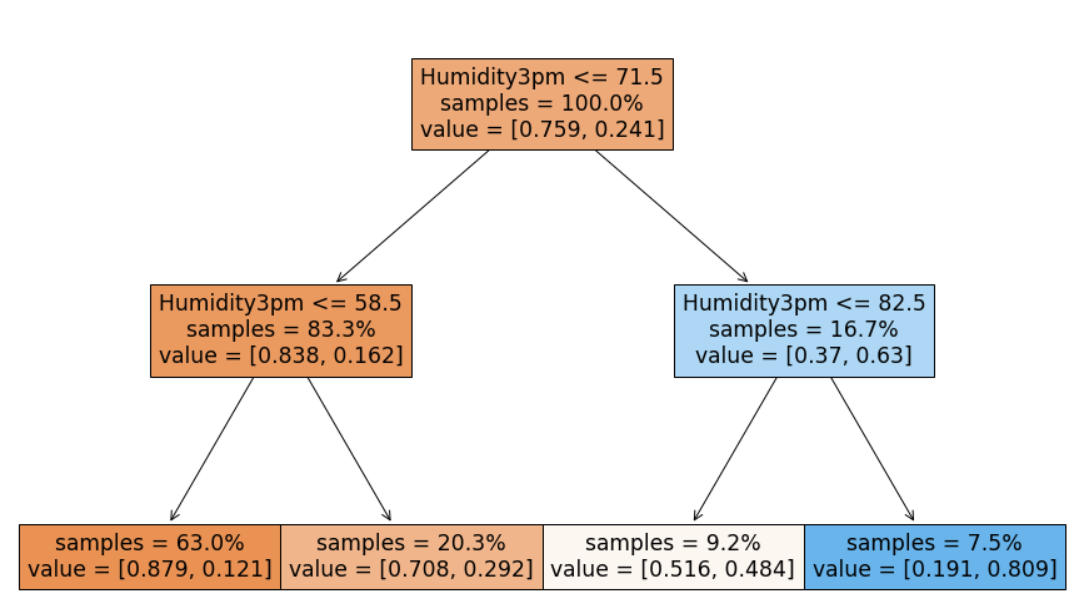
\includegraphics[width = 0.7\textwidth]{ex2_1_01}
	\caption{Árbol de decisión del Ejemplo \ref{Ej:2.1}}
	\label{fig:Ejemplo 2.1}
\end{figure}

Como se puede observar, el algoritmo es muy intuitivo: a  partir de la información de un individuo, se considera la primera condición; si la respuesta es afirmativa se sigue el camino de la izquierda y si es negativa el de la derecha. Mediante este proceso, se va comprobando si sus variables explicativas cumplen las diferentes condiciones que se plantean hasta alcanzar un grupo al que no se le aplican condiciones, el cual determinará su predicción. En los nodos de la Figura \ref{fig:Ejemplo 2.1}, se presenta la información relativa al porcentaje de individuos presentes en cada uno y la proporción de individuos de cada clase (atributo \textit{value}). Así, sabemos que los 3 primeros nodos hoja devolverán una respuesta negativa mientras que el último clasificará a sus individuos en la clase afirmativa.

Por otro lado, es fácil ver que las condiciones del algoritmo se corresponden con particiones del espacio. Como en el ejemplo anterior se han elegido únicamente dos variables explicativas, se puede hacer una representación de los individuos sobre $\mathbb{R}^{2}$ y determinar sobre él las diferentes regiones de predicción. En la Figura \ref{fig:Ejemplo 2.1.2} se puede observar la partición del espacio del ejemplo mencionado. Cabe destacar que esta partición se basa en una única línea vertical ya que, como se puede apreciar en la Figura \ref{fig:Ejemplo 2.1}, la variable ``Cloud3pm'' no ha sido seleccionada en el árbol para ninguna de las escisiones y un único nodo hoja clasificará a sus individuos en la clase ``Sí''.
\begin{figure}[h]
	\centering
	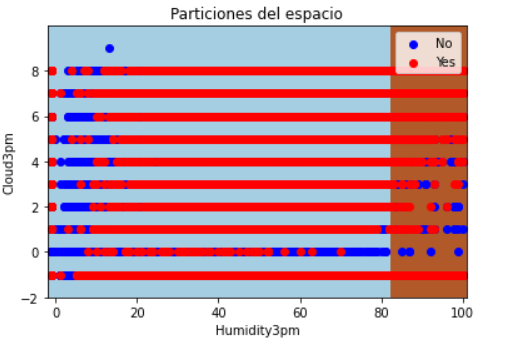
\includegraphics[width = 0.5\textwidth]{ex2_1_02}
	\caption{Partición del espacio del Ejemplo \ref{Ej:2.1}}
	\label{fig:Ejemplo 2.1.2}
\end{figure}


\subsubsection{Notación y conceptos básicos}

A continuación, se introducen una serie de términos básicos para poder hacer referencias correctas a los conceptos presentados. Por un lado, nos encontramos con las siguientes definiciones:
\begin{description}
\item[Nodo raíz: ]Primer nodo, contiene a todos los individuos y a partir de él comienzan a realizarse las divisiones.
\item[Nodo interno: ]Nodos intermedios que provienen de una división y desencadenan otra. Dentro de ellos, se pueden definir:
	\begin{description}
	\item[Nodo padre: ]Nodo anterior a un nodo interno fijado.
	\item[Nodos hijos: ]Nodos resultantes de la división del nodo interno fijado.
	\end{description}
\item[Nodo hoja: ]Nodos finales que dan lugar a la predicción.
\end{description}

Todos estos elementos son fácilmente identificables en la figura \ref{fig:Ejemplo 2.1} del ejemplo 2.1 . Se tiene un nodo raíz, dos nodos internos y cuatro nodos hoja.

Por otro lado, conviene hablar del concepto de sobreajuste. Se dice que un modelo se encuentra sobreajustado si el algoritmo se ha adaptado en exceso a los individuos del conjunto de entrenamiento. Este hecho provoca que la predicción de los individuos de este conjunto sea muy buena, pero que las predicciones de nuevos individuos presenten grandes errores.

%Para lidiar con el sobreajuste, interesa manejar otras dos nociones: el sesgo y la varianza. El sesgo (en inglés: \textit{bias}) hace referencia a los errores cometidos en las predicciones de los individuos del conjunto de entrenamiento. Por contra, la varianza es la medida del error cometido en los individuos que no pertenecen a este conjunto. En el trabajo, la varianza será medida en los individuos del conjunto de testeo. Estos conceptos plantean un problema: interesa tener valores bajos de ambos indicadores, pero disminuir el sesgo conlleva un aumento de la varianza. Así, a la hora de construir un modelo de Machine Learning, interesa estudiar que el sesgo no sea excesivamente bajo, para evitar el sobreajuste, pero también que no sea excesivamente alto para que las predicciones sean fiables.


\subsubsection{Objetos de estudio de un CART}

Una vez explicada, de manera intuitiva, la manera de proceder de los árboles de decisión, corresponde explicar el verdadero funcionamiento de los mismos. Para ello, habrá que tratar los siguientes aspectos:
\begin{enumerate}
\item Elección de variables y valores asociados a cada nodo interno.
\item Criterio de parada de división de los nodos
\item Valor o clase asignada a cada nodo
\end{enumerate}



\subsection{Valor o clase asignada a cada nodo hoja} \label{sec:2.4}
Sea un conjunto de datos de $n$ individuos y $p+1$ variables ($n,p \in \mathbb{N}$). Sean $X_1, X_2, ... , X_p$ las variables explicativas e $Y$ la variable dependiente. En el caso del conjunto de datos de ejemplo:
\begin{table}[h]
\centering
\begin{tabular}{l|l|l|l|l|l|}
\cline{2-6}
                                                       & \cellcolor[HTML]{C0C0C0}$X_1$ & \cellcolor[HTML]{C0C0C0}$X_2$ & \cellcolor[HTML]{C0C0C0}$\dots$ & \cellcolor[HTML]{C0C0C0}$X_{22}$ & \cellcolor[HTML]{9B9B9B}$Y$ \\ \hline
\multicolumn{1}{|l|}{\cellcolor[HTML]{C0C0C0}$1$}    & 2008-12-01                    & Albury                        & $\dots$                         & No                               & No                          \\ \hline
\multicolumn{1}{|l|}{\cellcolor[HTML]{C0C0C0}$2$}    & 2008-12-02                    & Albury                        & $\dots$                         & No                               & No                          \\ \hline
\multicolumn{1}{|l|}{\cellcolor[HTML]{C0C0C0}$3$}     & 2008-12-02                    & Albury                        & $\dots$                         & No                               & No                          \\ \hline
\multicolumn{1}{|l|}{\cellcolor[HTML]{C0C0C0}$\vdots$} & $\vdots$                      & $\vdots$                      & $\ddots$                        & $\vdots$                         & $\vdots$                    \\ \hline
\end{tabular}
\caption{Datos \textit{``Rain in Australia''}}
\label{tab:Datos}
\end{table}

Se denotarán con minúscula los datos o valores concretos de cada individuo, siendo $(x_i, y_i)$ la fila $i$-ésima de la Tabla \ref{tab:Datos}.

Como se comentaba anteriormente, el resultado de un árbol de decisión es una partición del espacio. Si se obtienen $M$ regiones diferentes, denotadas por $R_{m}$ con $m = 1, ..., M$. Se define como $\hat{Y}$ al árbol de decisión y como $c_m$ a las predicciones (imágenes de $\hat{Y}$) asociadas a cada región $R_m$. De este modo:
\begin{equation*}
\hat{Y}(x) = \sum^M_{m = 1} c_{m}I(x \in R_m) \, \, \, \forall x \in D
\end{equation*}

\noindent
donde $D$ es el dominio de la función $\hat{Y}$ (espacio de las variables explicativas) e $I$ es la función indicadora:
\begin{equation*}
I(x) = 
\left\{
\begin{array}{ccc}
1 & si & x \in R_m \\
0 & si & x \not\in R_m 
\end{array}
\right.
\end{equation*}

La manera de establecer el valor de estas predicciones presenta ligeras diferencias en función del tipo de problema con el que se trate (regresión o clasificación). Por tanto, se analizarán por separado.


\subsubsection{Árboles de regresión}
En un modelo de regresión, se busca minimizar los errores entre $Y$ e $\hat{Y}$. Tomando el error mínimo cuadrático, se llega al problema:
\begin{equation*}
\min_{\hat{Y}_i} \sum_{i=1}^n (y_i - \hat{Y}_i)^2 \Rightarrow \min_{c_m} \sum_{m = 1}^M \sum_{x_i \in R_m} (y_i - c_m)^2
\end{equation*}

\noindent
donde $\hat{Y}_i = \hat{Y}(x_i) \, \, \forall i=1,...n$. Denotando $f(c_m) = \sum_{x_i \in R_m} (y_i - c_m)^2$, se observa que alcanzar la solución óptima del problema planteado es equivalente a minimizar la función $f$. Derivando, se obtiene un candidato a óptimo:
\begin{equation}
\label{eq:01}
f'(c_m) = -2 \sum_{x_i \in R_m} (y_i - c_m) = -2 \sum_{x_i \in R_m}y_i + 2n_mc_m = 0 \Leftrightarrow c_m = \frac{1}{n_m} \sum_{x_i \in R_m}y_i
\end{equation}

\noindent
y se comprueba que, efectivamente, es el óptimo a través de la segunda derivada:
\begin{equation*}
f''(c_m) = -2 \sum_{x_i \in R_m} (-1) = 2n_m > 0
\end{equation*}

\noindent
donde $n_m$ es el conjunto de datos pertenecientes a la región $R_m$, $\forall m = 1,...M$.

En conclusión, el valor asignado a cada nodo hoja será la media de las observaciones de los individuos del conjunto de entrenamiento que pertenecen a dicho nodo.


\subsubsection{Árboles de clasificación}

En el caso de árboles de clasificación, la tarea se simplifica: basta con calcular la proporción de individuos de cada clase en cada región y, así, el valor asignado a cada subconjunto del espacio será la clase a la que le corresponde la mayor proporción en el mismo.


\subsection{Elección de variables y valores asociados a cada nodo interno} \label{sec: subsec22}
\subsubsection{Árboles de regresión}
Se analizará la primera división y el proceso será similar para las siguientes. Al situarse en el nodo raíz, se pretende dividir el conjunto de datos inicial en dos regiones, denotadas por $R_1$ y $R_2$, en función de una de las variables explicativas, $X_j$, y de un valor respecto de ésta, $s$, de manera que cada región contendrá a los individuos:
\begin{equation*}
R_1 (j,s) = \{ x_i | x_{ij} \leq s \} \, \, \, \wedge \, \, \,  R_2 (j,s) = \{ x_{i} | x_{ij} > s\}
\end{equation*}

Así, se generan dos valores de predicción constantes, uno por cada nodo hoja; es decir, se definen $c_1$ y $c_2$ tales que $c_1$ se mantendrá constante sobre $R_1$ y $c_2$ constante sobre $R_2$, calculados según (\ref{eq:01}). De esta manera, se buscan $j$ y $s$ que minimicen:
\begin{equation*}
\min_{j,s} \left( \sum_{x_i \in R_1}(y_i - c_1)^2 + \sum_{x_i \in R_2}(y_i - c_2)^2 \right)
\end{equation*}

\noindent
o lo que es lo mismo, se buscan $j$ y $s$ que minimicen la suma de residuos cuadráticos (RSS, del inglés: \textit{``Residuals Sum of Squares''}) en el conjunto de entrenamiento.

Así, a la hora de dividir el nodo raíz, se comprueban todas las posibles divisiones posibles y se escogen $j$ y $s$ óptimos. A continuación, se aplica el mismo proceso recursivamente para los nodos hijos generados.


\subsubsection{Árboles de clasificación}
En el caso de los árboles de clasificación, la variable dependiente es una clase. Es decir, la situación es equivalente a la recogida en la Tabla \ref{tab:Datos}. En este caso, se utiliza una función de impureza que permita evaluar la homogeneidad de los nodos; o lo que es lo mismo, que permita estudiar qué acciones separan mejor el espacio en función de las diferentes clases. El criterio más empleado es el índice Gini, que se define de la forma:
\begin{equation*}
G_{region\_m} = G_m = \sum_{k=1}^K p_{mk}(1 - p_{mk})
\end{equation*}

\noindent
donde $p_{mk}$ es la proporción de individuos del conjunto de entrenamiento de clase $k$ que se encuentran en la región $m$ y $K$ es el número total de clases. Además, se puede observar que valores de $p_{mk}$ cercanos a 0 o 1 implican que el producto $p_{mk}(1- p_{mk})$ sea muy pequeño. Por tanto, el índice Gini actúa como medidor de la pureza de una región: un índice Gini de bajo valor significa que los diferentes $p_{mk}$ están cercanos a 0 o 1 y la región es ``pura''.

Para evaluar el índice Gini asociado a la división de un nodo se utiliza una media ponderada de los índices de las dos regiones generadas tras la escisión, es decir:
\begin{equation*}
G_{nodo} = \frac{n_1}{n_1 + n_2}G_1 + \frac{n_2}{n_1 + n_2}G_2
\end{equation*}

\noindent
donde  $n_1$ y $n_2$ son el número de individuos de las regiones $R_1$ y $R_2$, respectivamente, y $G_1$ y $G_2$ son los índices Gini de las mismas. 

Por tanto, al igual que en los árboles de regresión, la tarea se resume en obtener, mediante comprobación de todas las opciones posibles, la variable y el valor que minimizan el índice Gini del nodo y aplicar el proceso recursivamente.




\subsection{Criterio de parada de escisión de nodos}
Es lógico pensar que la precisión de un árbol CART aumenta conforme aumenta en profundidad (número de divisiones). No obstante cuantas más particiones del espacio realice el algoritmo, mayor será el ajuste del mismo a los datos de entrenamiento, lo que puede llevar a problemas de \textit{overfitting}. Con tal de evitar estos problemas, se han implementado algunos métodos de ``poda'' del árbol (eliminación de algunas de las divisiones realizadas). Es evidente que podando el árbol se introduce sesgo, pues no se permite que se ajuste totalmente a los datos; sin embargo, aplicando estos procesos de manera controlada se consigue disminuir la varianza y mejorar las predicciones.

Por un lado, la técnica más simple consiste en establecer una profundidad máxima del árbol, es decir, poner límite a la cantidad de nodos hijo a desarrollar. Con esta condición, se puede asegurar que los nodos dejarán de dividirse una vez alcanzado el nivel indicado. Por ejemplo, en el Ejemplo \ref{Ej:2.1} se ha establecido una profundidad máxima igual a 2.

Por otro lado, el árbol determinará un nodo como nodo hoja cuando la separación del mismo no sea conveniente en términos de pureza. El procedimiento es el siguiente: en primer lugar, se calcula el índice Gini de la región asociada a ese nodo y, después, se realiza la mejor división del nodo y se calcula el índice Gini del mismo (proveniente de la media ponderada de índices de sus regiones). Si el índice de la región sin dividir es inferior al índice del nodo, se deshará la división y se determinará el nodo como nodo hoja, pues su división no mejora la pureza.





\subsection{Ejemplo} \label{ex:CART}
\emph{Se desea obtener una predicción fiable acerca de las precipitaciones del día siguiente en una ciudad de Australia. El objetivo es realizar una clasificación en ``lluvia'' o ``no lluvia''. Para ello, haciendo uso del dataset anteriormente introducido, se dividirá el conjunto de datos en dos subconjuntos: uno de entrenamiento y otro de testeo. Además, se probará con diferentes profundidades máximas permitidas para escoger el modelo más fiable. En particular, se construirán árboles de profundidades 1, 3, 5, 10, 15, 20 y 30.}

\begin{table}[H]
\centering
\includegraphics[width = 0.39\textwidth]{ex2_2_01}
\caption{Coeficientes de Gini en 7 árboles de clasificación para los datos ``Rain in Australia''}
\label{tab:exCART}
\end{table}

\emph{En la Tabla \ref{tab:exCART} se ven reflejados el tiempo de ejecución de cada árbol, los coeficientes de Gini para los conjuntos de entrenamiento y testeo y el porcentaje de información que se pierde en el conjunto de testeo respecto del de entrenamiento. Como se puede observar, cuando la profundidad máxima permitida es superior o igual a 10, el modelo empieza a sobreajustarse a los datos de entrenamiento, aumentando la desviación entre los conjuntos conforme aumenta la profundidad máxima permitida. Así, los modelos más fiables son el $DT\_3$ y el $DT\_5$ (profundidades 3 y 5) pues en ambos la variación se encuentra por debajo del $5\%$. En la Figura \ref{fig:exCART} se puede comprobar que estos modelos son los óptimos ya que permitiendo una mayor profundidad se obtiene una precisión menor con una diferencia mayor entre conjuntos.}


\begin{figure}[h]
\centering
\includegraphics[width = 0.5\textwidth]{ex2_2_02}
\caption{Evolución de los coeficientes Gini en ambos conjuntos}
\label{fig:exCART}
\end{figure}

\newpage
\emph{Intuitivamente, el valor $delta\%$ se puede entender como desviación que sufre el conjunto de testeo con el paso de 2 años (los datos de testeo van de 2015 a 2017). Por tanto, si se escogiese un modelo con un $delta\% = 20\%$, tendríamos que este $20\%$ se iría incrementando en las predicciones cada dos años, algo que llevaría a un modelo totalmente impreciso. Por ello, se escogen aquellos con variaciones pequeñas.}

\emph{Por último, nótese que el tiempo empleado en la generación de los árboles presentados es mínimo. Los modelos escogidos ($DT_3$ y $DT_5$) apenas tardan medio segundo en construirse, resultado que es prueba de la eficiencia de esta clase de modelos.}





\subsection{Ventajas y desventajas}
\textbf{\underline{Ventajas:}}
\begin{itemize}
\item Válidos para problemas de regresión y de clasificación.
\item Válidos para una exploración inicial de los datos.
\item Modelos de bajo coste computacional.
\item Método muy intuitivo de fácil comprensión, sencillo de comunicar a compañeros no expertos.
\item La manera de proceder del modelo se asemeja a cómo lo hace la mente humana: se van estableciendo condiciones que restringen, paso a paso, el conjunto total de datos hasta llegar a la solución.
\item Se puede obtener una representación gráfica de los diferentes modelos, lo cual facilita su comprensión a nivel visual.
\end{itemize}

\textbf{\underline{Desventajas:}}
\begin{itemize}
\item La capacidad predictora de los árboles de decisión es inferior a la que se puede obtener mediante otros métodos. De hecho, podemos observar que los coeficientes de Gini de los modelos del Ejemplo \ref{ex:CART} en el conjunto de testeo no alcanza el $65\%$.
\item Se trata de un algoritmo inestable. Es decir, un ligero cambio en los datos de entrenamiento puede conllevar a la creación de un modelo totalmente distinto. %¿Por qué?
\item Con un árbol de decisión es ineficiente modular correlaciones lineales altas entre la variable objetivo y una variable explicativa. Modular esta alta correlación podría ser más eficiente con un modelo clásico de Regresión Lineal o Logística.
\end{itemize}


No obstante, pese a no poseer una gran capacidad de predicción, existen diferentes maneras de combinar árboles de decisión de forma que se obtengan modelos de mayor precisión y que no se sobreajusten.




\newpage
\section{Métodos derivados de los árboles de decisión}
Tanto CART como muchos de los algoritmos utilizados para construir árboles de decisión se desarrollaron a lo largo de la década de los 80. No obstante, ya se ha visto en el Ejemplo \ref{ex:CART} que estos algoritmos no llegan a alcanzar grandes niveles de precisión; es por eso que a partir de la década de los 90 empiezan a surgir diferentes artículos que introdujeron nuevas técnicas que, mediante distintas combinaciones de árboles de decisión, consiguen modelos de mayor fiabilidad y que incorporan distintas características que los convierte en modelos muy potentes. A la hora de combinar los árboles de decisión para construir modelos más complejos se pueden seguir dos caminos: bagging o boosting. Dedicaremos esta sección al estudio de ambos.


\subsection{Algoritmos de bagging}

Los algoritmos de bagging (\textit{``Bootstrap Aggregation''}) se caracterizan por tomar muestras aleatorias del conjunto de datos inicial y construir con ellas árboles de decisión diferentes. Se analizarán tres algoritmos de bagging distintos: Bagging, Random Forest y Extra-Trees.


\subsubsection{Bagging}
Tras participar en la creación del algoritmo CART, Leo Breiman publicó, en 1996, un artículo en el que introducía un nuevo método con el fin de disminuir la varianza de CART: Bagging \cite{BR01}. Bagging es un algoritmo que toma diferentes muestras aleatorias de individuos con repetición del conjunto de datos y con cada una de ellas construye un árbol de decisión haciendo uso de todas las variables explicativas disponibles. De esta manera, se consiguen diferentes predicciones, todas ellas del mismo peso, a través de las cuales se obtiene una respuesta final mediante el cálculo de la media (regresión) o mediante conteo de clases, escogiendo la clase con más apariciones (clasificación).


\subsubsection{Random Forest}
El desarrollo de Bagging llevó a Breiman a definir un nuevo algoritmo 5 años más tarde. Con Random Forest \cite{BR02}, Breiman consiguió, además de disminuir la varianza, obtener información más completa de las variables explicativas. El procedimiento es muy parecido al de Bagging: nuevamente, se toman diferentes muestras con repetición de los individuos y, para cada muestra, también se toma una muestra aleatoria de $m$ variables (con $m \leq p$). Una buena elección de $m$ podría ser: $ m = \lfloor \sqrt{p} \rfloor$.

Por tanto, la diferencia con Bagging es que ahora cada árbol se construirá teniendo en cuenta una muestra aleatoria de las variables explicativas. De esta manera, dado que en ocasiones tenemos variables muy correlacionadas con la variable a predecir, se consigue que no siempre sean estas variables las que participen en el modelo y, así, participe el máximo número de variables posibles en la respuesta final.


\subsubsection{Extra-Trees} \label{sec:ExtraTrees}
El algoritmo Extra-Trees, o \textit{Extremely Randomized Trees}, aporta aún más margen a la aleatoriedad dentro del modelo. Utiliza como base lo descrito en Random Forest, pero presenta una particularidad en cuanto a la escisión de nodos. Como se explica en la subsección \ref{sec: subsec22}, en la escisión de nodos se busca la variable, y el valor óptimo asociado, que minimizan una función de error o impureza. En Extra-Trees, en lugar de probar todos los valores posibles de todas las variables disponibles, se generará un valor aleatorio de corte para cada una de las variables que será el que se evalúe. Así, se probará con $m$ valores aleatorios correspondientes a las $m$ variables explicativas escogidas al azar. En particular, este algoritmo puede resultar muy útil ante problemas de \textit{overfitting} extremos.


\subsubsection{Error de Out-Of-Bag}
Cabe dedicar un apartado para hablar de la noción del error \textit{Out-Of-Bag} (OOB). Como ya se ha visto, los algoritmos de bagging toman muestras con repetición de los individuos para la construcción de cada uno de los árboles. Aquellos individuos que no participan en la creación de un árbol reciben el nombre de individuos \textit{out-of-bag}. Si se cuenta con $n$ individuos, la probabilidad de que un individuo no se escoja para la creación de un árbol (individuo \textit{out-of-bag}) es:
\begin{equation*}
\left( \frac{n-1}{n} \right)^n
\end{equation*}

Por tanto, se puede observar que cuando el número de invididuos de la muestra sea elevado (supóngase $n \rightarrow +\infty$):
\begin{equation*}
\lim_{n \rightarrow + \infty} \left( \frac{n-1}{n} \right)^n = \lim_{n \rightarrow +\infty} \left( 1 - \frac{1}{n} \right)^n = \lim_{n \rightarrow +\infty} \left[ \left( 1 + \frac{1}{-n} \right)^{-n} \right] ^{-1} = e^{-1} \simeq 0.3679
\end{equation*}

Es decir, si se trabaja con un conjunto de datos de gran tamaño, cerca de un $37 \%$ de los individuos no se tendrán en cuenta para la creación de cada árbol (en particular). Así, en bagging, el error del modelo se puede evaluar en el conjunto OOB, que actúa como conjunto test. Para cada árbol del modelo, los individuos que se utilizarán para el testeo serán aquellos individuos \textit{out-of-bag} del árbol en cuestión. Además, una propiedad muy buena del error OOB es que converge a medida que se añaden árboles al modelo. De esta manera, podemos asegurar que los modelos de bagging no se sobreajustan.

No obstante, en los ejemplos se seguirá evaluando la precisión del modelo empleando la validación \textit{Out Of Time}. El motivo es el ya comentado en la subsección \ref{subsec:Metodología}: interesa realizar una separación de ``datos pasados'' y ``datos futuros'' y los individuos \textit{out-of-bag} son aleatorios dentro del conjunto de entrenamiento.


%QUEDA PENDIENTE ENUNCIAR EL TEOREMA EXACTO (¿Y DEMOSTRARLO?).


\subsubsection{Ejemplo} \label{ex:Bag}
\emph{Nuevamente, se desea predecir si lloverá o no el próximo día en una ciudad de Australia haciendo uso, ahora, de los algoritmos de bagging. Además, con tal de evitar sobreajustes, se establecerá el criterio de parada de los árboles generados en 5 (como se ve en el Ejemplo \ref{ex:CART}, es el más fiable junto a 3) y se probará con diferentes números de árboles generados por cada algoritmo.}

\begin{table}[h]
\centering
\includegraphics[width = \textwidth]{ex3_1_01}
\caption{Resultados algoritmos de bagging para RainTomorrow: a)Bagging b)Random Forest c)Extra-Trees}
\label{tab:exbagging}
\end{table}

\emph{Aplicando los diferentes algoritmos se llega a los resultados expuestos en la Tabla \ref{tab:exbagging}. Como se puede apreciar, la mejora respecto a CART es evidente: en el ejemplo anterior se llegaba a la conclusión de que una de las mejores opciones era elegir el árbol con profundidad máxima 5 que otorgaba una precisión en Gini del 66$\%$ en el conjunto de entrenamiento y del 63$\%$ en el de testeo. Ahora, tanto en Bagging como en Random Forest, escogiendo cualquiera de los modelos que realiza al menos 10 árboles, se obtienen coeficientes de Gini que rozan, en ocasiones, el 70$\%$ en ambos conjuntos. En el caso de Extra-Trees, la mejora no es tan significativa pero los coeficientes siguen siendo mejores. Además, en los tres modelos se aprecia un sustancial descenso, de aproximadamente 1 punto porcentual, en delta, lo cual refleja una clara disminución de la varianza del modelo. }

\emph{También, se puede observar que el modelo no se sobreajusta al incrementar el número de estimadores que se generan; y que este incremento no produce grandes cambios en los coeficientes de Gini a partir de un cierto número de árboles. Así, el error converge como se puede comprobar visualmente en la Figura \ref{fig:exbagging}.}

\begin{figure}[h]
\centering
\includegraphics[width = 0.8 \textwidth]{ex3_1_02}
\caption{Convergencia coeficientes Gini}
\label{fig:exbagging}
\end{figure}

\emph{Por último, nótese que los algoritmos de bagging son más costosos que CART en cuanto al tiempo empleado para su construcción. Además, se puede observar una clara relación entre los diferentes modelos y el tiempo que requieren. A la hora de construir los árboles de decisión, Bagging tiene en cuenta todas las variables, Random Forest solo considera algunas de ellas y Extra-Trees, además de no usar todas las variables, evalúa las posibles escisiones de nodos en base a valores aleatorios. Estas características se ven claramente reflejadas en los tiempos de ejecución, pues los tiempos de ejecución más altos corresponden a Bagging y los más bajos se le atribuyen a Extra-Trees.}


\subsubsection{Ventajas y desventajas}
\textbf{\underline{Ventajas:}}
\begin{itemize}
\item  Algoritmos capaces de disminuir la varianza; lo que implica que las predicciones realizadas serán (casi) igual de fiables que las del conjunto de entrenamiento.
\item Aumento de precisión respecto a otros algoritmos más simples (como CART).
\item Al tratarse de modelos ``democráticos'', son buenas alternativas estables en problemas con datos ruidosos, con bajas correlaciones o con datos faltantes.
\end{itemize}

\textbf{\underline{Desventajas:}}
\begin{itemize}
\item Se pierde la fácil visualización y comprensión de CART.
\item Pese a la mejora en la precisión, el nivel de fiabilidad sigue siendo relativamente pobre (en el Ejemplo \ref{ex:Bag} no se alcanza el $70 \%$ de precisión en Gini).
\end{itemize}



\subsection{Algoritmos de boosting}
Los algoritmos de boosting, al igual que los de bagging, generan diferentes árboles de decisión a través de los cuales se realiza la predicción final. No obstante, mientras los algoritmos de bagging generan árboles independientes y devuelven una respuesta promedio o la respuesta más votada, los algoritmos de boosting generan los árboles secuencialmente, teniendo en cuenta los resultados anteriores. De esta manera, esta clase de métodos consigue un significativo descenso del sesgo ya que la forma en la que se construyen los diferentes árboles permite otorgar pesos diferentes a los individuos, consiguiendo así que el nuevo árbol generado se focalice en predecir bien a aquellos individuos que presentan mayor error (o que se han clasificado erróneamente) en el árbol anterior.

A lo largo de esta subsección trataremos de abordar a fondo los principales algoritmos de boosting: AdaBoost, Gradient Boosting, XGBoost, LightGBM y CatBoost.


\subsubsection{AdaBoost} \label{sec:AdaBoost}
Adaboost (\textit{``\textbf{Ada}ptative \textbf{Boost}ing''}) \cite{FR01} es un algoritmo que construye árboles de decisión con solo dos nodos hoja; es decir, con una sola escisión, por lo que está pensado para ser ejecutado con un alto número de iteraciones. A estos árboles de decisión se les llamará ``tocones''. En la figura \ref{fig: AdaBoost_01} se puede observar un ejemplo de estos árboles.
\begin{figure}[h]
\centering
\includegraphics[width = 0.3\textwidth]{AdaBoost_01_1}
\caption{Ejemplo de tocón construido en AdaBoost.}
\label{fig: AdaBoost_01}
\end{figure}

En la práctica, AdaBoost construye un primer tocón a partir de todos los datos disponibles, cuyo resultado es considerado como la predicción inicial del modelo, y a continuación se realiza un cálculo de errores respecto a esta predicción. Así, se genera un nuevo conjunto de datos a través de una muestra con repetición del conjunto inicial, en la que tendrán mayor probabilidad de aparecer aquellos individuos con errores más altos. Después, la siguiente y sucesivas iteraciones consistirán en construir nuevos tocones que clasifiquen la muestra de datos correspondiente a la iteración, calculando los errores pertinentes y los sucesivos conjuntos de datos. De esta manera, AdaBoost construye una cadena de árboles donde se le resta importancia a la predicción de aquellos individuos para los que ya ha conseguido errores bajos mientras que aumenta el peso de los individuos mal predichos para que sean el principal objetivo en los árboles posteriores. Por último, la respuesta final del modelo será la predicción inicial más las predicciones de las sucesivas iteraciones. A continuación, se procederá a explicar de manera detallada el algoritmo ``Discrete AdaBoost''. Éste fue el primer algoritmo presentado en el que se hace referencia a este método, y aborda problemas de clasificación binaria. 

En el primer paso, se asigna el mismo peso a todos los individuos. Así, en primer lugar:
\begin{equation*}
w_i = \frac{1}{n} \, \, \, \forall i \in \{1, \dots, n \}
\end{equation*}

En cada una de las $M$ iteraciones, se crea un tocón, denotado por $\hat{Y}_m(x)$ con $m \in \{1, \dots, M \}$. Además, dado que estos árboles solo poseen dos nodos hoja, en cada tocón únicamente se verá involucrada una variable.

El error de la iteración $m$-ésima se calcula de la forma:

\begin{equation*}
err_m = \frac{\sum_{i=1}^{n} w_i I(y_i \neq \hat{y}_{i, m})}{\sum_{i=1}^{n} w_i} 
\end{equation*}

\noindent
con $\hat{y}_{i, m} = \hat{Y}_m(x_i)$, es decir, la suma de los pesos de los individuos mal clasificados en el numerador y la suma total de los pesos en el denominador. Dado que Adaboost tiene diferentes implementaciones, en algunas de ellas el denominador puede ser distinto de 1. No obstante, siguiendo la implementación de Python, siempre se estandarizarán los pesos antes de empezar de nuevo con el bucle, por lo que se puede considerar el denominador igual a 1:

\begin{equation*}
err_m = \frac{\sum_{i=1}^{n} w_i I(y_i \neq \hat{y}_{i, m})}{\sum_{i=1}^{n} w_i} = \frac{\frac{1}{n} \sum_{i=1}^{n}I(y_i \neq \hat{y}_{i, m})}{1} = \frac{num.errores}{n}
\end{equation*}

A continuación, se calcula el coeficiente:

\begin{equation*}
\alpha _m = \log \left( \frac{1 - err_m}{err_m} \right)
\end{equation*}

Como se puede observar, si el tocón $\hat{Y}_m(x)$ ha realizado un buen trabajo de clasificación ($err_m \simeq 0$), a $\alpha_m$ le corresponderá un valor positivo. Por el contrario, un mal trabajo de clasificación ($err_m \simeq 1$) se verá traducido en un $\alpha_m$ negativo. Así, se puede entender $\alpha_m$ como un medidor de la importancia del tocón $\hat{Y}_m(x)$ en el modelo: un valor alto implica una buena clasificación general y, por tanto, su respuesta es importante para el resultado final y, por otro lado, un valor bajo implica una clasificación general pobre con un número considerable de errores y conviene que su influencia en el resultado final no sea muy elevada. Esta evolución del $\alpha_m$ en función del error se puede comprobar visualmente en el gráfico de la función expuesto en la Figura \ref{fig: AdaBoost_02}.

\begin{figure}[h]
\centering
\includegraphics[width = 0.5\textwidth]{AdaBoost_02}
\caption{Gráfico de $\alpha_m$}
\label{fig: AdaBoost_02}
\end{figure}

Al final de cada iteración, se recalculan los pesos a través de la expresión:
\begin{equation*}
w_i^{m+1} =
\left\{
\begin{array}{crl}
w_i^m & si & y_i = \hat{y}_{i, m} \\
w_i^m e^{\alpha_m} & si & y_i \neq \hat{y}_{i, m} \\
\end{array}
\right.
\end{equation*}

\noindent
donde $w_i^m$ es el peso del individuo $i$ en la iteración $m$-ésima. Nótese que en caso de que $\hat{Y}_m(x)$ haga un buen trabajo de clasificación ($\alpha_m \ggg 0$) habrá pocos individuos mal clasificados y a $e^{\alpha_m}$ le corresponderá un valor alto; pues, dado que $\hat{Y}_m(x)$ tendrá una importancia relevante en el modelo, interesa priorizar la correcta clasificación de aquellos que han presentado errores. Conforme $\alpha_m$ se va acercando a 0, la importancia del tocón en el modelo disminuye, efecto que se ve reflejado en la modificación de los pesos pues $e^{\alpha_m}$ se acercará a 1 y no habrá apenas diferencia entre los pesos de la iteración actual y su consecutiva. Por otro lado, en caso de que $\hat{Y}_m(x)$ tenga una eficacia del $50\%$, $\alpha_m = 0$, el modelo no tendrá importancia y, dado que la probabilidad de acertar o no es la misma, no tiene sentido modificar los pesos. Por último, en el caso de obtener un modelo $\hat{Y}_m(x)$ que haga un pésimo trabajo de clasificación (eficacia menor que el $50\%$), $\alpha_m \lll 0$, se podría interpretar que el modelo está trabajando a la inversa y que hay que considerar las clasificaciones contrarias que éste proporciona. Por tanto, en este caso, interesa disminuir el peso de los mal clasificados por el modelo, lo que es equivalente a aumentar el peso de los bien clasificados, ya que los que el modelo clasifique correctamente serán los que serán considerados como erróneos dada la eficacia del modelo.

Finalizando con las iteraciones, queda hacer especial hincapié en un par de conceptos. Se puede observar en la sección \ref{sec: subsec22} que en la expresión del índice Gini dada para escisión de nodos no intervienen los pesos de los individuos. No obstante, en AdaBoost es necesario que los tocones se construyan teniendo en cuenta los pesos de los individuos. La solución más fácil, y la que se encuentra implementada en la librería \emph{Scikit-learn} de Python, es la siguiente: se estandarizan los pesos, es decir, se divide el peso de cada individuo por la suma total de pesos, y se considera el resultado como las frecuencias relativas de cada individuo. Así, se pueden conseguir también las frecuencias absolutas de la muestra. Se pueden observar los pasos descritos en la Tabla \ref{tab:AdaB_pesos}.
\begin{table}[h]
\centering
\begin{tabular}{|c|c|}
\hline
Individuo & w \\ \hline
1 & $w_1$ \\ \hline
2 & $w_2$ \\ \hline
\vdots & \vdots \\ \hline
n & $w_n$ \\ \hline
\end{tabular}
$\Rightarrow$
\begin{tabular}{|c|c|}
\hline
Individuo & w* \\ \hline
1 & $\frac{w_1}{\sum_{i=1}^n w_i}$ \\ \hline
2 & $\frac{w_2}{\sum_{i=1}^n w_i}$ \\ \hline
\vdots & \vdots \\ \hline
n & $\frac{w_n}{\sum_{i=1}^n w_i}$ \\ \hline
\end{tabular}
$\Rightarrow$
\begin{tabular}{|c|c|}
\hline
Individuo & w* \\ \hline
1 & $w_1^*$ \\ \hline
2 & $w_2^*$ \\ \hline
\vdots & \vdots \\ \hline
n & $w_n^*$ \\ \hline
\end{tabular}
$\Rightarrow$
\end{table}
\begin{table}[h]
\centering
$\Rightarrow$
\begin{tabular}{|c|c|c|}
\hline
Individuo & w* & F\\ \hline
1 & $w_1^*$ & $w_1^*$ \\ \hline
2 & $w_2^*$ & $\displaystyle \sum_{i=1}^2 w_i^*$ \\ \hline
\vdots & \vdots & \vdots \\ \hline
n & $w_n^*$ & $\displaystyle \sum_{i=1}^n w_i^* \, \, (= 1)$ \\ \hline
\end{tabular}
$\Rightarrow$
\begin{tabular}{|c|c|}
\hline
Individuo & F \\ \hline
1 & $F_1$ \\ \hline
2 & $F_2$ \\ \hline
\vdots & \vdots \\ \hline
n & $F_n \, \, (=1)$ \\ \hline
\end{tabular}
\caption{Reasignación de pesos}
\label{tab:AdaB_pesos}
\end{table}

El siguiente paso es generar $n$ números aleatorios $(t_1, t_2, \dots, t_n)$ pertenecientes al intervalo [0, 1]. Entonces, se cumple que:
\begin{equation*}
\exists j \in \{1, \dots, n \} /t_i \in [F_{j-1}, F_{j}] \, \, \forall i \in \{1, \dots, n \}
\end{equation*}
donde $F_0$ = 0.

Así, la solución propuesta al problema de los pesos consiste en crear un nuevo conjunto de datos utilizando los $t_i$ generados aleatoriamente: si $t_i \in [F_{j-1}, F_{j}]$, entonces se añade $x_j$ al nuevo conjunto. De esta manera, se obtiene un nuevo conjunto de datos de $n$ individuos en el que los individuos mal clasificados por el árbol anterior tendrán mayor presencia (como sus pesos son más altos, los intervalos $[F_{j-1}, F_{j}]$ serán más amplios). Por último, se asigna un peso de $1/n$ a cada uno de los individuos del nuevo conjunto de datos y ya se procede a la creación del siguiente tocón.


\textbf{\underline{Ejemplo funcionamiento del bucle:}}

\textit{Supóngase que el conjunto de datos se redujese al de la Tabla \ref{tab:AdaBoost_03}.}
\begin{table}[H]
\centering
\includegraphics[width = 0.3\textwidth]{AdaBoost_03}
\caption{Submuestra del conjunto de datos para ilustrar el funcionamiento del bucle.}
\label{tab:AdaBoost_03}
\end{table}

\textit{Inicialmente, se crea un árbol de decisión de una única división, obteniendo el tocón y la consiguiente partición del espacio ilustrados en la figura \ref{fig:AdaBoost_04}.}

\begin{figure}[h]
\centering
\includegraphics[width = 0.5\textwidth]{AdaBoost_04}
\caption{Primer tocón del modelo}
\label{fig:AdaBoost_04}
\end{figure}

\textit{Como se puede observar, solo hay un individuo mal clasificado, el número 9. A continuación, se calcula $err_1$:}
\begin{equation*}
err_1 = \frac{num.errores}{n} = \frac{1}{10} = 0.1
\end{equation*}

\noindent
\textit{y, haciendo uso de él, se obtiene $\alpha_1$:}
\begin{equation*}
\alpha_1 = \log{\frac{1 - err_1}{err_1}} = \log{\frac{1- 0.1}{0.1}} = \log{\frac{0.9}{0.1}} = \log{9} \simeq 2.1972
\end{equation*}

\textit{Una vez hechos estos cálculos, se realiza la reasignación de pesos:}
\begin{equation*}
w_i^{m+1} =
\left\{
\begin{array}{crl}
w_i^m & si & y_i = \hat{y}_{i, m} \\
w_i^m e^{\alpha_m} & si & y_i \neq \hat{y}_{i, m} \\
\end{array}
\right.
\Rightarrow
w_i^{2} =
\left\{
\begin{array}{crl}
w_i^1 & si & i \neq 9 \\
w_i^1 e^{\alpha_1} & si & i = 9 \\
\end{array}
\right.
\Rightarrow
w_i^{2} =
\left\{
\begin{array}{crl}
w_i^1 & si & i \neq 9 \\
9 w_i^1  & si & i = 9 \\
\end{array}
\right.
\end{equation*}

\noindent
\textit{donde los superíndices hacen referencia a la iteración. Así, modificados los pesos, se aplica el proceso recogido en la Tabla \ref{tab:AdaB_pesos} y se obtienen los resultados de la Tabla \ref{tab:AdaB_pesos_ex}. }
\begin{table}[h]
\centering
\begin{tabular}{|c|c|}
\hline
Individuo & $w^2$ \\ \hline
0 & $0.1$ \\ \hline
1 & $0.1$ \\ \hline
2 & $0.1$ \\ \hline
3 & $0.1$ \\ \hline
4 & $0.1$ \\ \hline
5 & $0.1$ \\ \hline
6 & $0.1$ \\ \hline
7 & $0.1$ \\ \hline
8 & $0.1$ \\ \hline
9 & $0.9$ \\ \hline
\end{tabular}
$\Rightarrow$
\begin{tabular}{|c|c|}
\hline
Individuo & $w^{2^*}$ \\ \hline
0 & $\frac{0.1}{1.8}$ \\ \hline
1 & $\frac{0.1}{1.8}$ \\ \hline
2 & $\frac{0.1}{1.8}$ \\ \hline
3 & $\frac{0.1}{1.8}$ \\ \hline
4 & $\frac{0.1}{1.8}$ \\ \hline
5 & $\frac{0.1}{1.8}$ \\ \hline
6 & $\frac{0.1}{1.8}$ \\ \hline
7 & $\frac{0.1}{1.8}$ \\ \hline
8 & $\frac{0.1}{1.8}$ \\ \hline
9 & $\frac{0.9}{1.8}$ \\ \hline
\end{tabular}
$\Rightarrow$
\begin{tabular}{|c|c|}
\hline
Individuo & $w^{2^*}$ \\ \hline
0 & $0.0556$ \\ \hline
1 & $0.0556$ \\ \hline
2 & $0.0556$ \\ \hline
3 & $0.0556$ \\ \hline
4 & $0.0556$ \\ \hline
5 & $0.0556$ \\ \hline
6 & $0.0556$ \\ \hline
7 & $0.0556$ \\ \hline
8 & $0.0556$ \\ \hline
9 & $0.5$ \\ \hline
\end{tabular}
$\Rightarrow$
\end{table}

\begin{table}[H]
\centering
$\Rightarrow$
\begin{tabular}{|c|c|}
\hline
Individuo & F \\ \hline
0 & $0.0556$ \\ \hline
1 & $0.1111$ \\ \hline
2 & $0.1667$ \\ \hline
3 & $0.2222$ \\ \hline
4 & $0.2778$ \\ \hline
5 & $0.3333$ \\ \hline
6 & $0.3889$ \\ \hline
7 & $0.4444$ \\ \hline
8 & $0.5$ \\ \hline
9 & $1$ \\ \hline
\end{tabular}
\caption{Transformación del peso en frecuencias}
\label{tab:AdaB_pesos_ex}
\end{table}

\textit{Por tanto, solo queda generar 10 números aleatorios en [0, 1] y asociarlos a los individuos en función del intervalo en el que se encuentren, tal y como se muestra en la Tabla \ref{tab:AdaB_selec}.}
\begin{table}[H]
\centering
\begin{tabular}{|c|c|c|c|c|c|c|c|c|c|c|}
\hline
t & 0.3954 & 0.4193 & 0.0144 & 0.5211 & 0.0210 & 0.9923 & 0.0953 & 0.5072 & 0.7743 & 0.8238 \\ \hline
Fila & 7 & 7 & 0 & 9 & 0 & 9 & 1 & 9 & 9 & 9 \\ \hline
\end{tabular}
\caption{Selección de individuos para el nuevo conjunto de datos}
\label{tab:AdaB_selec}
\end{table}

\textit{Por tanto, el conjunto de datos que utilizaremos para entrenar el segundo tocón será el formado por los individuos que aparecen en la Tabla \ref{tab:AdaB_selec}. Como se puede comprobar, el individuo 9, antes mal clasificado, ahora aparece 5 veces, por lo que el algoritmo tendrá que clasificarlo bien para no asumir un error tan elevado.}

\bigskip \bigskip


Una vez terminado el bucle, queda analizar cómo realiza las predicciones AdaBoost. La solución del algoritmo es:
\begin{equation*}
\hat{Y}(x) = sign \left[ \sum_{m=1}^M \alpha_m \hat{Y}_m(x) \right]
\end{equation*}

Entonces, dado que el algoritmo ``Discrete AdaBoost'' se diseñó para resolver problemas de clasificación binaria, a una clase se le asocia el valor $-1$ y a la otra el valor $+1$. Por tanto, la respuesta será la siguiente: si $\sum_{m=1}^M \alpha_m \hat{Y}_m(x) < 0$, $\hat{Y}(x) = - 1$; y en caso de $\sum_{m=1}^M \alpha_m \hat{Y}_m(x) > 0$, $\hat{Y}(x) = 1$. De esta manera, como ya se avanzaba anteriormente, $\alpha_m$ es un medidor de la importancia del tocón dentro del modelo, pues un $\alpha_m$ alto implicará una gran contribución de la respuesta del tocón a la respuesta final.

\bigskip

\textbf{\underline{Consideraciones finales AdaBoost:}}

Tras la publicación de ``Discrete AdaBoost'', se expuso el algoritmo ``Real Adaboost'' \cite{FR02}, que extendía el funcionamiento del algoritmo visto al caso continuo y a más de dos grupos. A continuación, analicemos qué modificaciones se añaden para afrontar problemas de clasificación multiclase y problemas de regresión.

En el caso de tener más de dos grupos, en el último paso, la respuesta de la función será la clase cuyo sumatorio de $\alpha_m's$ sea mayor. Es decir, para cada clase $k$ se calcula $\sum_{m / \hat{Y}_m(x) = k} \alpha_m$ y la clase cuyo sumatorio sea mayor, es la que corresponde a la respuesta del algoritmo.
%Esto se puede desarrollar mucho mejor y más formal comentando lo de los J pares del artículo de Friedman et al.

En el caso de un problema de regresión, se utiliza una ``función de pérdida'' o, en inglés, \textit{``Loss Function''} (a partir de ahora, se hará referencia a ella en su término inglés dado que es como se conoce realmente). Esta función mide la discrepancia o distancia entre el verdadero valor $y_i$ y el valor $\hat{y}_i$ predicho por el modelo. Vendrá dada de la siguiente forma:
\begin{equation*}
L_i^{(m)} = L \left[ |\hat{y}^{(m)}(x_i) - y_i| \right] \, \, \, \, \forall i \in \{ 1, \dots, n \}
\end{equation*}

\noindent
donde $\hat{y}^{(m)}(x_i)$ hace referencia al valor predicho por el $m$-ésimo árbol al introducir los valores del individuo $i$-ésimo e $y_i$ es el valor de la variable dependiente en el individuo $i$-ésimo. Existen diferentes funciones candidatas Loss Function. De entre ellas, destacan las que devuelven valores entre $0$ y $1$, en concreto:
\begin{equation*}
\left\{
\begin{array}{cl}
L_i^{(m)} = \frac{|\hat{y}^{(m)}(x_i) - y_i|}{n} &  (lineal) \\ 
L_i^{(m)} = \frac{|\hat{y}^{(m)}(x_i) - y_i|^2}{n^2} & (cuadrada) \\
L_i^{(m)} = 1 - \exp \left[ \frac{-|\hat{y}^{(m)}(x_i) - y_i|}{n} \right] & (exponencial)
\end{array}
\right.
\end{equation*}

Una vez elegida la función a emplear, se calcula el error ponderado del tocón realizando la media de las $L_i^{(m)}$'s:
\begin{equation*}
L^{(m)} = \frac{1}{n}\sum_{i=1}^n L_i^{(m)}
\end{equation*}

De esta manera, se define el $\alpha_m$ en el caso de regresión de manera análoga a lo explicado anteriormente:
\begin{equation*}
\alpha_m = \log \left( \frac{1 - L^{(m)}}{L^{(m)}} \right)
\end{equation*}

Así, una vez solucionado el problema de cómo medir el error, el resto del procedimiento es análogo al de clasificación, tomando como respuesta final: $\hat{Y}(x) = \sum_{m = 1} ^M \alpha_m \hat{Y}_m(x)$.





\subsubsection{Gradient Boosting} \label{sec:GB}

Gradient Boosting \cite{FR03} es un algoritmo que, mediante la construcción secuencial de árboles, consigue identificar cuáles son aquellos individuos cuyos errores asociados son mayores y trata de mejorar las predicciones de los mismos. Al igual que AdaBoost, el primer paso consiste en determinar una predicción inicial. No obstante, mientras AdaBoost prosigue a través de actualizaciones de los pesos y de la generación de nuevos conjuntos de datos, Gradient Boosting construye una secuencia de árboles en la que cada árbol pretende corregir el error cometido por los árboles anteriores. Para ello, se requiere de una Loss Function a través de la cual obtiene los residuos y el valor asociado a cada nodo hoja de los árboles generados. El objetivo es minimizar esta Loss Function para, así, minimizar el error cometido. La respuesta final viene dada por la predicción inicial más la suma del resto de árboles que tratan de cuantificar los sucesivos errores. De esta forma, se parte de una predicción inicial con un error alto que se reduce iteración a iteración.

El algoritmo es el mismo tanto para el caso de regresión como para el de clasificación. La diferencia entre estos dos casos reside únicamente en la elección de la Loss Function a emplear. A continuación, se analizan ambos casos por separado. La notación empleada es la siguiente: $\hat{Y}_m(x)$ representa el árbol de decisión generado en la iteración $m$-ésima e $\hat{Y}^{(m)}(x)$ la $m$-ésima predicción, es decir: $\hat{Y}^{(m)}(x) = \displaystyle \sum_{k=1}^m \hat{Y}_k(x)$. Del mismo modo, $\hat{y}_{i,m} = \hat{Y}_m(x_i)$ e $\hat{y}_i^{(m)} = \hat{Y}^{(m)}(x_i)$.

\bigskip \bigskip 

\textbf{\underline{Regresión}}


Para iniciar el algoritmo, se debe establecer una Loss Function $L(y_i, \hat{y}_i)$. Ya se ha visto que existen diferentes funciones que pueden ser candidatas a Loss Function, por ello el algoritmo viene definido para una $L(y_i, \hat{y}_i)$ cualquiera. No obstante, en Gradient Boosting se suele hacer uso de:
\begin{equation*}
L(y_i, \hat{y}_i) = \frac{1}{2}(y_i - \hat{y}_i)^2
\end{equation*}

La elección de esta Loss Function se debe a que va a ser necesario derivarla. Así, derivando respecto de $\hat{y}_i$, la expresión resultante no es más que el residuo de la predicción:
\begin{equation}
\label{eq:02}
\frac{\partial L(y_i, \hat{y}_i)}{\partial \hat{y}_i} = -(y_i - \hat{y}_i)
\end{equation}

El primer paso consiste en determinar un valor fijo que representará la ``primera predicción''; es decir, aquella que luego será modificada en función de los residuos:
\begin{equation*}
\hat{Y}^{(0)}(x) = arg\min_{\gamma} \sum_{i=1}^N L(y_i, \gamma)
\end{equation*}

\noindent
siendo $\gamma = \hat{y_i}$. Sustituyendo por la función fijada queda:
\begin{equation*}
\hat{Y}^{(0)}(x) = arg\min_{\gamma} \sum_{i=1}^N L(y_i, \gamma) = arg\min_{\gamma} \frac{1}{2}\sum_{i=1}^N (y_i - \gamma)^2 
\end{equation*}

Ya se vio en la sección \ref{sec:2.4} (ecuación (\ref{eq:01})) que el valor de $\gamma$ que minimiza este valor es la media, por tanto:
\begin{equation*}
\hat{Y}^{(0)}(x) = \frac{1}{N} \sum_{i=1}^N y_i
\end{equation*}

A continuación, en cada una de las $M$ iteraciones de este bucle se genera un nuevo árbol que añadirá información a la última predicción realizada. Primero, se calcula el residuo de la última predicción de cada uno de los individuos(la $(m-1)$-ésima) mediante la derivada especificada en (\ref{eq:02}):
\begin{equation*}
r_{im} = - \left[ \frac{\partial L(y_i, \hat{y}_i)}{\partial \hat{y}_i} \right]_{\hat{y}_i = \hat{y}_i^{(m-1)}} = y_i -\hat{y}_i^{(m-1)}
\end{equation*}

Después, se genera un árbol cuyo objetivo es realizar una predicción de los residuos $r_{im}$ en función de las variables explicativas. Así, se denota por $R_{jm}$ a los diferentes nodos hoja del árbol $m$-ésimo y cada uno de ellos llevará asignado el valor de respuesta:
\begin{equation*}
\gamma_{jm} = arg\min_{\gamma} \sum_{x_i \in R_{jm}} L(y_i, \hat{y}_i^{(m-1)} + \gamma)
\end{equation*}

De nuevo, el $\gamma$ que minimizará dicha expresión será la media de los residuos de los individuos pertenecientes a $R_{jm}$. 

Para terminar con el bucle, se define cuál es la $m$-ésima actualización de la predicción:
\begin{equation*}
\hat{Y}^{(m)}(x) = \hat{Y}^{(m-1)}(x) + \nu \hat{Y}_m(x) = \hat{Y}^{(m-1)}(x) + \nu \sum_{j = 1}^{J_m}\gamma_{jm} I(x \in R_{jm})
\end{equation*}

\noindent
es decir, se le añade el residuo predicho a la última predicción calculada multiplicada por un valor $\nu \in [0, 1]$, donde $\nu$ es un parámetro, denominado ``tasa de aprendizaje'', que ayuda a evitar el sobreajuste. Como el algoritmo establece una predicción inicial que actualiza iteración a iteración haciendo uso de los residuos, la omisión de la tasa de aprendizaje implicaría un \textit{overfitting} en un número bajo de iteraciones. Cabe mencionar que Gradient Boosting se suele aplicar con $M$ grande y $\nu$ pequeño pues, en la práctica, se comprueba que es más fiable utilizar modelos que realicen muchos pasos de pequeñas modificaciones en lugar de pocos pasos de grandes modificaciones, pues tienden a sobreajustarse menos.

Por último, la respuesta del algoritmo es la de $\hat{Y}^{(M)}(x)$.

Cabe recordar que se ha desarrollado el algoritmo bajo la hipótesis de que la Loss Function escogida es la más habitual en este caso. Evidentemente, el procedimiento es análogo para cualquier función pero, en ese caso, valores como $\hat{Y}^{(0)}(x)$ o $\gamma_{jm}$ dejarán de ser medias y se tendrán que calcular los valores que minimizan las nuevas expresiones. Además, puntualizar que con otras funciones de pérdida no tienen por qué aparecer los valores $r_{im}$ como residuos, ya que la forma de estos podría ser muy diferente (no tendría por qué ser ``valor observado - valor predicho''). Es por eso que en Gradient Boosting se denomina a estos valores como ``pseudo-residuos''.



\bigskip \bigskip

\textbf{\underline{Clasificación: }}

El procedimiento está pensado para clasificación binaria. Ahora, el interés está en estimar la probabilidad de pertenecer a cierta clase de manera que si la probabilidad es mayor que 0.5 se clasificará en la clase ``1'' y si la probabilidad es menor que 0.5 se clasificará en la clase ``0''. No obstante, Gradient Boosting no aproxima esta probabilidad directamente, si no que aproxima el log-odd-ratio y, posteriormente, obtiene la probabilidad deseada:
\begin{equation*}
odd-ratio = \frac{p}{1-p}
\end{equation*}

En primer lugar, se verá cómo determinar la Loss Function escogida. Al tratarse de clasificación binaria, podemos considerar la v.a. $y_i$ cuya distribución de probabilidad es la bernoulli:
\begin{equation*}
f(y, p) = p^y(1-p)^{1-y}
\end{equation*}

Por tanto, la función de verosimilitud para una muestra de $n$ casos será:
\begin{equation*}
l(p|y_1, y_2, \dots, y_n) = \prod_{i=1}^n f_p(y_i) = \prod_{i=1}^n p^{y_i}(1-p)^{1-y_i}
\end{equation*}

\noindent
y la función soporte:
\begin{equation*}
ln(l(p)) = ln \left( \prod_{i=1}^n f_p(y_i) \right) = ln \left( \prod_{i=1}^n p^{y_i}(1-p)^{1-y_i} \right) = \sum_{i=1}^n y_i ln(p) + (1-y_i)ln(1-p)
\end{equation*}

Ahora, nótese que cuando se hace uso de esta función en el método de Máxima Verosimilitud, interesa maximizar su valor. Por el contrario, cuando trabajamos con una Loss Function, se trata de minimizarla, pues el modelo será más ajustado conforme menor sea el valor de esta función. Por tanto, si se desea emplear la función soporte como Loss Function, se tendrá que multiplicar por $-1$. También, como se desea aplicar esta función individuo a individuo, se puede eliminar el sumatorio. Así, la Loss Function queda:
\begin{equation*}
L(y_i, p_i) = -( y_i ln(p_i) + (1-y_i)ln(1-p_i))
\end{equation*}

No obstante, ésta es una función de $p_i$ y se desea trabajar con log-odd-ratio (a partir de ahora, por simplificar, $ln(odd_i)$). Entonces, se transforma esta expresión de la forma:
\begin{equation}
\label{eq:03}
\begin{split}
L(y_i, p_i) &= -(y_i ln(p_i) + (1-y_i)ln(1-p_i)) = -y_i ln(p_i) - ln(1-p_i) + y_i ln(1-p_i) = \\
& = -y_i(ln(p_i) - ln(1-p_i)) - ln(1-p_i) = -y_i ln \left( \frac{p_i}{1-p_i} \right) - ln(1-p_i) = \\
& = -y_i ln(odd_i) - ln(1-p_i)
\end{split}
\end{equation}

Además, se puede comprobar que $p_i = \frac{e^{ln(odd_i)}}{1 + e^{ln(odd_i)}}$ y así:
\begin{equation*}
ln(1-p_i) = ln \left( 1- \frac{e^{ln(odd_i)}}{1 + e^{ln(odd_i)}} \right) = ln \left( \frac{1}{1 + e^{ln(odd_i)}} \right) = - ln \left( 1 + e^{ln(odd_i)} \right)
\end{equation*}

Por tanto, volviendo a (\ref{eq:03}):
\begin{equation*}
L(y_i, p_i) = L(y_i, ln(odd_i)) = -y_i ln(odd_i) + ln \left( 1 + e^{ln(odd_i)} \right)
\end{equation*}

A continuación, se deben seguir los mismos pasos que en el caso de regresión pero sustituyendo por la nueva función. Como el procedimiento es, en la gran mayoría, análogo, se suprimirá parte de los desarrollos, disponibles en el Anexo (\ref{Anexo2}). 

Ahora, la predicción inicial vendrá dada por:
\begin{equation}
\label{eqn:1}
p_0(x) = arg\min_{\gamma} \sum_{i=1}^N L(y_i, \gamma) = arg\min_{\gamma} \sum_{i=1}^N \left( -y_i \gamma + ln \left( 1 + e^{\gamma} \right) \right) = \frac{\sum_{i=1}^{N} y_i}{N} 
\end{equation}

Se puede observar, dado que $y_i \in \{0, 1 \} \, \forall i \in \{1, \dots, n \}$, que la predicción inicial es la proporción de individuos del conjunto de entrenamiento que pertenecen a la clase ``1''. No obstante, dado que se quiere trabajar en términos de $ln(odd_i)$, se debe escribir esta probabilidad en la forma correspondiente. De esta manera:
\begin{equation*}
\hat{Y}^{(0)}(x) = \frac{p_0(x)}{1-p_0(x)} = \frac{\frac{\sum_{i=1}^{N} y_i}{N}}{1 - \frac{\sum_{i=1}^{N} y_i}{N}} = \frac{\sum_{i=1}^{N} y_i}{N -\sum_{i=1}^{N} y_i}
\end{equation*}

De acuerdo con lo anterior, el siguiente paso consiste en el bucle que calculará en cada iteración (supóngase la iteración $m$-ésima): los ``pseudo-residuos'' de la predicción $\hat{Y}_i^{(m-1)}(x)$, un árbol de decisión que clasifique estos residuos, los valores de respuesta de los nodos hoja del árbol generado y la nueva predicción $\hat{Y}^{(m)}(x)$.

Los ``pseudo-residuos'' vendrán dados por:
\begin{equation}
\label{eqn:2}
\begin{split}
r_{im} &= -\left[ \frac{\partial L(y_i, \hat{y}_i)}{\partial \hat{y}_i} \right]_{\hat{y}_i=\hat{y}_i^{(m-1)}} =  y_i - \frac{e^{\hat{y}_i^{(m-1)}}}{1 + e^{\hat{y}_i^{(m-1)}}}
\end{split}
\end{equation}

Nótese que $\hat{y}_i^{(m-1)}$ es, realmente, la última predicción realizada de $ln(odd_i)$. Por tanto, $r_{im}$ podría escribirse como:
\begin{equation*}
r_{im} = y_i - p_{i, m-1}
\end{equation*}

\noindent
donde $p_{i, m-1}$ es la predicción $(m-1)$-ésima de $p_i$, es decir, $r_{im}$ es $y_i$ menos la última predicción realizada del mismo.

A continuación, se construye un árbol de decisión que realice una predicción de los pseudoresiduos en función de las variables independientes y se denotan sus nodos hoja por $R_{jm}$ con $j \in \{1, \dots, J_m \}$, donde $J_m$ es el número total de nodos hoja del $m$-ésimo árbol. Dada la hoja (o región) $j$, la predicción de los individuos pertenecientes a $R_{jm}$ vendrá dada por:
\begin{equation*}
\gamma_{jm} = arg\min_{\gamma} \sum_{x_i \in R_{jm}} L(y_i, \hat{y}_i^{(m-1)} + \gamma)
\end{equation*}

Para obtener el valor de $\gamma$ que minimiza dicha expresión, se aproxima $L(x_i, \hat{y}_i^{(m-1)} + \gamma)$ mediante su desarollo de Taylor de segundo orden, pues en este caso no resulta sencillo derivar e igualar a $0$. Se hará para un $i$ cualquiera con el fin de no complicar los cálculos con los sumatorios. Es decir, se considera:
\begin{equation*}
L(y_i, \hat{y}_i^{(m-1)} + \gamma) \approx L(y_i, \hat{y}_i^{(m-1)}) + \frac{d}{d(ln(odd_i))}L(y_i, \hat{y}_i^{(m-1)})\gamma + \frac{1}{2}\frac{d^2}{d(ln(odd_i))^2}L(y_i, \hat{y}_i^{(m-1)})\gamma^2
\end{equation*}

\noindent
y se deriva respecto de $\gamma$ igualando a cero puesto que es lo que se busca minimizar:
\begin{equation*}
\begin{split}
\frac{d}{d\gamma}L(y_i, \hat{y}_i^{(m-1)} + \gamma) &\approx \frac{d}{d(ln(odd_i))}L(y_i, \hat{y}_i^{(m-1)}) + \frac{d^2}{d(ln(odd_i))^2}L(y_i, \hat{y}_i^{(m-1)})\gamma \, \, \Rightarrow \\
& \Rightarrow \, \, \gamma = - \frac{\frac{d}{d\hat{y}_i^{(m-1)}}L(y_i, \hat{y}_i^{(m-1)})}{\frac{d^2}{(d\hat{y}_i^{(m-1)})^2}L(y_i, \hat{y}_i^{(m-1)})}
\end{split}
\end{equation*}

Realizando el cálculo de estas derivadas se obtiene:
\begin{equation}
\label{eqn:3}
\gamma = \frac{y_i - \frac{e^{\hat{y}_i^{(m-1)}}}{1 + e^{\hat{y}_i^{(m-1)}}}}{\frac{e^{\hat{y}_i^{(m-1)}}}{(1 + e^{\hat{y}_i^{(m-1)}})^2}}
\end{equation}

Además, realizando las transformaciones adecuadas, se llega a que esta expresión es equivalente a:
\begin{equation}
\label{eqn:4}
\gamma = \frac{y_i - p_{i, m-1}}{p_{i, m-1}(1 - p_{i, m-1})}
\end{equation}

Para finalizar con los cálculos, recuérdese que se ha decidido omitir los sumatorios en el desarrollo realizado. Ahora bien, como la derivada de un sumatorio es igual al sumatorio de las derivadas, se puede afirmar que:
\begin{equation*}
\gamma_{jm} = \frac{\displaystyle \sum_{x_i \in R_{jm}} y_i - \frac{e^{\hat{y}_i^{(m-1)}}}{1 + e^{\hat{y}_i^{(m-1)}}}}{\displaystyle \sum_{x_i \in R_{jm}} \frac{e^{\hat{y}_i^{(m-1)}}}{(1 + e^{\hat{y}_i^{(m-1)}})^2}} = \frac{\displaystyle \sum_{x_i \in R_{jm}} y_i - p_{i, m-1}}{\displaystyle \sum_{x_i \in R_{jm}} p_{i, m-1}(1 - p_{i, m-1})}
\end{equation*}

A partir de aquí el procedimiento es equivalente al visto en el caso de Gradient Boosting para regresión: se actualiza el valor de la predicción $(m-1)$-ésima a partir de los $\gamma_{jm}$ y la predicción final será la predicción $M$-ésima, es decir, la correspondiente a la última iteración del bucle.

Por último, cabe recordar que en este caso estamos realizando predicciones de log-odd-ratio; por tanto, para obtener la probabilidad deseada y clasificar en una clase o en la otra, habrá que llevar a cabo la transformación:
\begin{equation*}
p = \frac{e^{ln(odd)}}{1 + e^{ln(odd)}}
\end{equation*}





\subsubsection{XGBoost} \label{sec:XGBoost}
XGBoost(\textit{'e\textbf{X}treme \textbf{G}radient \textbf{Boost}ing'}) \cite{CH01} es un algoritmo que utiliza de base lo explicado en la última sección añadiendo una serie de mejoras que lo convierten en una herramienta muy potente. Actualmente, es uno de los modelos cuyo dominio es imprescindible y su continuada aparición entre los finalistas de concursos de Machine Learning dan fe de su importancia y utilidad.

Este algoritmo utiliza la misma idea de Gradient Boosting: generar árboles de decisión que realicen predicciones secuenciales de los residuos. No obstante, presenta una serie de modificaciones entre las que destacan la manera de construir los árboles y la inclusión de parámetros de regularización, como $\lambda$ y $\gamma$, que ayudan a evitar el sobreajuste restando importancia a los datos aislados y aportando aleatoriedad. Además, XGBoost fue diseñado para trabajar con conjuntos de datos muy grandes, por lo que estos parámetros de regularización serán de ayuda, sobretodo, en el caso de que el conjunto de datos no sea lo suficientemente grande.

A continuación, al igual que se realizó en Gradient Boosting, se explicarán el caso de regresión y el de clasificación por separado.



\bigskip \bigskip

\textbf{\underline{Regresión}}

En el caso de regresión, la Loss Function elegida es la misma que se escogió en Gradient Boosting:
\begin{equation*}
L(y_i, \hat{y}_i) = \frac{1}{2}(y_i - \hat{y}_i)^2
\end{equation*}

El primer paso consiste en definir la predicción inicial, denotada por $\hat{Y}^{(0)}$. Como ya se ha visto en cálculos anteriores (sección \ref{sec:GB}), esta primera predicción vendrá dada por:
\begin{equation*}
\hat{Y}^{(0)}(x) = \frac{1}{N} \sum_{i=1}^N y_i
\end{equation*}

A continuación, interviene un bucle de $M$ iteraciones en el que, en cada iteración, se genera un árbol que predice los residuos respecto de la última predicción calculada. Así para la $m$-ésima iteración calculamos, de manera análoga a los $r_{im}$ de Gradient Boosting:
\begin{equation*}
g_{m}(x_i) = \left[ \frac{\partial L(y_i, \hat{y}_i)}{\partial \hat{y}_i} \right]_{\hat{y}_i = \hat{y}_i^{(m-1)}} = \hat{y}_i^{(m-1)} - y_i
\end{equation*}

Por otro lado, también será necesario conocer el valor de la segunda derivada. Se tiene:
\begin{equation*}
h_{m}(x_i) = \left[ \frac{\partial^2 L(y_i, \hat{y}_i)}{\partial \hat{y}_i^2} \right]_{\hat{y}_i = \hat{y}_i^{(m-1)}} = 1
\end{equation*}

A continuación se genera un árbol de decisión que clasifique los residuos. La respuesta de estos árboles vendrá dada por los valores $\omega_j$ (valor asociado al $j$-ésimo nodo hoja) que minimicen la siguiente función:
\begin{equation*}
\mathcal{L}^{(m)} = \sum_{i=1}^n L(y_i, \hat{y}_i^{(m-1)} + \hat{y}_{i,m}) + \gamma T + \frac{1}{2}\lambda \sum_{j=1}^T \omega_j^2
\end{equation*}

\noindent
donde $\gamma$ y $\lambda$ son parámetros de regularización. $\mathcal{L}^{(m)}$ es la Loss Function que se utilizará para la construcción de los árboles. Actúa como función de perdida ya que utiliza la función previamente introducida pero además incorpora los parámetros de regularización mencionados. Para minimizar esta función se recurre al desarrollo de Taylor de segundo orden de $L(y_i, \hat{y}_i^{(m-1)} + \hat{y}_{i,m})$ de manera que:
\begin{equation*}
\mathcal{L}^{(m)} \approx \sum_{i=1}^n \left( L(y_i, \hat{y}_i^{(m-1)}) + g_m(x_i)\hat{y}_{i, m} + h_m(x_i)\hat{y}_{i, m}^2 \right)  + \gamma T + \frac{1}{2}\lambda \sum_{j=1}^T \omega_j^2
\end{equation*}

Ahora, teniendo en cuenta que $ \displaystyle \sum_{i=1}^n \hat{y}_{i, m} = \sum_{j = 1}^T\sum_{i \in I_j} \omega_j$ con $I_j = \{ i \, / \, x_i \in R_j \}$ y eliminando los términos que se mantienen constantes, la expresión anterior se puede reescribir de la forma:
\begin{equation*}
\mathcal{L}^{(m)} \approx \sum_{j = 1}^T \left( (\sum_{i \in I_j} g_m(x_i))\omega_j + \frac{1}{2}(\sum_{i\in I_j} h_m(x_i) + \lambda)\omega_j^2 \right) + \gamma T
\end{equation*}

Así, derivando respecto de $\omega_j$ e igualando a 0 se tiene que:
\begin{equation*}
\omega_j^* = - \frac{\sum_{i \in I_j} g_m(x_i)}{\sum_{i \in I_j} h_m(x_i) + \lambda} = - \frac{\sum_{i \in I_j} \hat{y}_i^{(m-1)} - y_i}{\sum_{i \in I_j} 1 + \lambda}
\end{equation*}

\noindent
expresión que se puede interpretar como $\frac{\sum_{i \in I_j} Residuos_i}{Num\_Residuos_j + \lambda}$. De esta manera, se observa que para nodos hoja formados por muchos residuos, el efecto del parámetro $\lambda$ será mínimo y el $\omega_j$ se corresponderá, prácticamente, con la media de los valores del nodo. Esto es porque, para $N_j$ (número de residuos del $j$-ésimo nodo hoja) grande:
\begin{equation*}
\omega_j^* = \frac{\sum_{i \in I_j} Residuos_i}{N_j + \lambda} = \frac{\sum_{i \in I_j} Residuos_i}{N_j} \times \frac{N_j}{N_j + \lambda} \approx \frac{\sum_{i \in I_j} Residuos_i}{N_j}
\end{equation*}

Así, $\lambda$ actúa como parámetro de regularización ya que modifica considerablemente la respuesta de aquellos nodos hoja a los que corresponden pocos individuos; es decir, la respuesta de las observaciones aisladas. Aumentar $\lambda$ implica disminuir los pesos y aumentar su coste en la Loss Function. En resumen, escogiendo un $\lambda \ggg 0$ se reduce el \textit{overfitting}.

Una vez visto qué valor asignar a los nodos hoja de los árboles que se construyen en XGBoost, veamos la profundidad que alcanzan estos árboles. Para ello, sustituyendo el valor $\omega_j^*$ en la ecuación de $\mathcal{L}^{(m)}$ se obtiene:
\begin{equation*}
\mathcal{L}^{*(m)} = - \frac{1}{2} \sum_{j = 1}^T \frac{\left( \sum_{i \in I_j} g_m(x_i) \right)^2}{\sum_{i \in I_j} h_m(x_i) + \lambda} + \gamma T 
\end{equation*}

El criterio de escisión de nodos de los árboles se basará en esta última fórmula. Dado un nodo $I$, se realiza una división de manera que $I = I_L \cup I_R$, donde $I_L$ hace referencia al nodo hijo izquierdo e $I_R$ al derecho. Así, se define una función de ganancia (\textit{``Gain''}) que realiza un trabajo análogo al realizado por la función de impureza explicada en CART (sección \ref{sec: subsec22}):
\begin{equation*}
Gain_I = \frac{G_I}{H_I} = \frac{\left( \sum_{i \in I} g_m(x_i) \right)^2}{\sum_{i \in I} h_m(x_i) + \lambda}
\end{equation*}

Entonces, las variables y los valores escogidos como referencia para la escisión serán aquellos que maximicen la función:
\begin{equation*}
\begin{split}
\mathcal{L}_{split} &= \frac{1}{2} \left( Gain_{I_L} + Gain_{I_R} - Gain_{I} \right) - \gamma = \frac{1}{2} \left( \frac{G_{I_L}}{H_{I_L}} + \frac{G_{I_R}}{H_{I_R}} - \frac{G_I}{H_I} \right) - \gamma = \\
&= \frac{1}{2} \left( \frac{\left( \sum_{i \in I_L} g_m(x_i) \right)^2}{\sum_{i \in I_L} h_m(x_i) + \lambda} + \frac{\left( \sum_{i \in I_R} g_m(x_i) \right)^2}{\sum_{i \in I_R} h_m(x_i) + \lambda} - \frac{\left( \sum_{i \in I} g_m(x_i) \right)^2}{\sum_{i \in I} h_m(x_i) + \lambda} \right)   - \gamma
\end{split}
\end{equation*}

\noindent
y el criterio de escisión será dividir en caso de que $\mathcal{L}_{split} > 0$ y no dividir en caso de que $\mathcal{L}_{split} < 0$. En este criterio, se puede apreciar la función de parámetro de regularización que realiza $\gamma$, ya que cuanto mayor sea el $\gamma$, menor será la probabilidad de dividir el nodo. De esta manera, para $\gamma \ggg 0$, los árboles generados no serán muy profundos y se evitará el sobreajuste; y para $\gamma \simeq 0$, los árboles se generarán de manera parecida a CART: si la ganancia de los nodos hijos es mayor que la del nodo padre, se divide.

En particular, dada la Loss Function fijada:
\begin{equation*}
\mathcal{L}_{split} = \frac{1}{2} \left( \frac{\left( \sum_{i \in I_L} \hat{y}_i^{(m-1)} - y_i \right)^2}{\sum_{i \in I_L} 1 + \lambda} + \frac{\left( \sum_{i \in I_R} \hat{y}_i^{(m-1)} - y_i \right)^2}{\sum_{i \in I_R} 1 + \lambda} - \frac{\left( \sum_{i \in I} \hat{y}_i^{(m-1)} - y_i \right)^2}{\sum_{i \in I} 1 + \lambda} \right)   - \gamma
\end{equation*}

Una vez explicado como genera los árboles XGBoost, el resto del procedimiento es análogo a Gradient Boosting. La predicción realizada por el árbol $m$-ésimo se añade a la última predicción realizada(la $(m-1)$-ésima) y se toma como predicción final del modelo $\hat{Y}^{(M)}(x)$.



\bigskip

\textbf{\underline{Clasificación}}

Al igual que en Gradient Boosting, la Loss Function que se suele emplear en XGBoost es:
\begin{equation*}
L(y_i, ln(odd_i)) = -y_i ln(odd_i) + ln \left( 1 + e^{ln(odd_i)} \right)
\end{equation*}

Ahora, las derivadas de la iteración $m$-ésima serán:
\begin{equation*}
g_m(x_i) = -y_i + \frac{e^{\hat{y}_i^{(m-1)}}}{1 + e^{\hat{y}_i^{(m-1)}}} \, \, \, \, \wedge \, \, \, \, h_m(x_i) = \frac{e^{\hat{y}_i^{(m-1)}}}{(1 + e^{\hat{y}_i^{(m-1)}})^2}
\end{equation*}

\noindent
que se pueden escribir en términos de las probabilidades predichas $p_{i, m-1}$ (visto en Gradient Boosting):
\begin{equation*}
g_m(x_i) = -y_i + p_{i, m-1} \, \, \, \, \wedge \, \, \, \, h_m(x_i) = p_{i, m-1}(1 - p_{i, m-1})
\end{equation*}

Así, para obtener el criterio de escisión de nodos seguido en la construcción de los árboles se deben sustituir estos valores en:
\begin{equation*}
\mathcal{L}_{split} = \frac{1}{2} \left( \frac{\left( \sum_{i \in I_L} g_m(x_i) \right)^2}{\sum_{i \in I_L} h_m(x_i) + \lambda} + \frac{\left( \sum_{i \in I_R} g_m(x_i) \right)^2}{\sum_{i \in I_R} h_m(x_i) + \lambda} - \frac{\left( \sum_{i \in I} g_m(x_i) \right)^2}{\sum_{i \in I} h_m(x_i) + \lambda} \right)   - \gamma 
\end{equation*}

\noindent
y para obtener el valor de los $\omega_j^*$ basta con sustituir en:
\begin{equation*}
\omega_j^* = - \frac{\sum_{i \in I_j} g_m(x_i)}{\sum_{i \in I_j} h_m(x_i) + \lambda}
\end{equation*}

\noindent
mientras que el resto del procedimiento es análogo.

De nuevo, cabe tener en cuenta que la predicción vendrá dada en términos de log-odd-ratio, por lo que habrá que realizar la transformación:
\begin{equation*}
p = \frac{e^{ln(odd)}}{1 + e^{ln(odd)}}
\end{equation*}

\noindent
para obtener la probabilidad deseada y clasificar.

\bigskip \bigskip

\textbf{\underline{Otras optimizaciones}}

Además de la particular forma que tiene XGBoost de construir los árboles, también incluye otra serie de mecanismos que hacen de él una herramienta muy potente. A continuación, se explicará, sin entrar en muchos detalles, cuáles son estos métodos que aplica.

Por un lado, como XGBoost se ideó para conjuntos de datos muy grandes, a la hora de realizar las escisiones de los árboles, probar con todos los valores posibles de todas las variables para determinar cuáles maximizan la función $\mathcal{L}_{split}$ conllevaría un gasto computacional inasumible. Así, una manera eficaz de llevar a cabo esta tarea es probar solo con los percentiles de cada variable. Por ejemplo, tomando los percentiles $P_{25}$, $P_{50}$ y $P_{75}$, solo habrá que probar con 3 valores por variable y escoger el óptimo. En la práctica, se suelen usar alrededor de 33 percentiles. Además, estos percentiles están ponderados; esto quiere decir que no todos los intervalos recogen el mismo número de individuos, sino que la suma de los pesos de los individuos es igual en todos los intervalos. El peso de cada individuo en la iteración $m$-ésima viene dado por $h_m(x_i)$ que, como ya se ha visto:
\begin{equation*}
h_m(x_i) = 1 \, \, \, \, \vee \, \, \, \, h_m(x_i) = p_{i, m-1}(1 - p_{i, m-1})
\end{equation*}

\noindent
según se trate de un problema de regresión o de clasificación, respectivamente. Así, en el caso de regresión los percentiles se calculan de la forma habitual y en el caso de clasificación se tendrán en cuenta las últimas predicciones realizadas. La idea intuitiva de por qué los pesos vienen dados por $h_m(x_i)$ pasa por observar que se puede reescribir la ecuación de $\mathcal{L}^{(m)}$ como:
\begin{equation*}
\mathcal{L}^{(m)} = \sum_{i = 1}^n \frac{1}{2} h_m(x_i) \left( f_m(x_i) - \frac{g_m(x_i)}{h_m(x_i)} \right)^2 + \Omega(f_m) + constant
\end{equation*}

\noindent
con $\Omega(f_m)$ los términos de regularización, de manera que se puede interpretar considerando $h_m(x_i)$ el peso del individuo y el otro factor como una función de pérdida.

Por otro lado, XGBoost es capaz de trabajar con conjuntos de datos con datos ausentes (o \textit{``Null values''}) sin necesidad de depurarlos previamente. Cuando se construyen los árboles para predecir los residuos, a la hora de separar un nodo, si se tienen variables con datos vacíos, para cada uno de los valores que se le otorguen a la variable para analizar el valor de \textit{``Gain''} se contemplarán dos casos: que los residuos de aquellos datos vacíos se encuentren en el nodo hijo izquierdo y que se encuentren en el derecho. De esta manera, el algoritmo tendrá en cuenta más particiones pero seguirá escogiendo aquella que maximice la ganancia y, por tanto, se podrán predecir resultados sin necesidad de conocer el valor de todas las variables explicativas.

Por último, también se tienen en cuenta ciertas mejoras desde el punto de vista de la implementación. Con la intención de optimizar el tiempo de computación, XGBoost recurre a diferentes técnicas: 
\begin{itemize}
\item \textbf{Paraleliza el conjunto de datos} enviando fragmentos del mismo a diferentes terminales.

\item \textbf{Calcula $g_m(x_i)$ y $h_m(x_i)$ haciendo uso de la memoria RAM} para realizar las operaciones necesarias en el menor tiempo posible.

\item \textbf{Realiza una compresión del conjunto de datos} ya que es más eficiente comprimirlos y descomprimirlos que leerlos directamente del disco duro. Además, en caso de disponer de más de un disco duro, separa el conjunto entre los disponibles con la finalidad de ganar velocidad.
\end{itemize}



\subsubsection{LightGBM}

LightGBM (del inglés: \textit{\textbf{Light} \textbf{G}radient \textbf{B}oosting \textbf{M}achine}) \cite{CH02} es un algoritmo desarrollado por Microsoft que fue publicado en 2017. Su funcionamiento es similar al de XGBoost pero añadiendo una serie de matices que consiguen obtener modelos muy potentes y eficientes.

La diferencia principal reside en el modo de construir los árboles. Como se puede observar en la Figura \ref{fig:LGBM}, en cada capa de nodos, XGBoost realiza la división de todos ellos (\textit{Level-wise tree growth}) y luego evalúa si dicha evaluación se debe llevar a cabo a través del valor de \textit{``Gain''}. Por el contrario, LightGBM no trabaja por capas (\textit{Leaf-wise tree growth}) sino que, a la hora de generar un árbol de decisión, se decide separar el nodo raíz y luego, de los dos nodos resultantes, sólo se separará el nodo que maximice la ganancia. Así, en la siguiente iteración, se contará con tres nodos que podremos dividir y, de nuevo, se valorará cuál de los tres maximiza la ganancia y será dividido. Por tanto, en cada iteración de la construcción del árbol, se calculará la ganancia de cada escisión y solo se realizará aquella que la maximice.

\begin{figure}[h]
\centering
\includegraphics[width = 0.4\textwidth]{LGBM_01}
\caption{Construcción de árboles en LightGBM vs XGBoost (Fuente: \cite{MA01})}
\label{fig:LGBM}
\end{figure}


Además de esta particularidad de LightGBM, también se aplican diferentes modificaciones computacionales que mejoran el tiempo de ejecución considerablemente, consiguiendo a veces una mejor precisión que XGBoost en un tiempo menor. Por ejemplo, LightGBM está diseñado para ser muy veloz al hacer uso de la CPU, procesador presente en todos los ordenadores. Por el contrario, XGBoost obtiene mejores resultados de tiempo al trabajar con la GPU, procesador gráfico que no poseen todos los equipos. Por tanto, al trabajar en CPU ambos, los tiempos de ejecución de LightGBM son mejores que los de XGBoost.



\subsubsection{CatBoost} \label{sec:CatBoost}

CatBoost \cite{DO01} es un modelo desarrollado por Yandex también publicado en 2017. Al igual que LightGBM, guarda gran parecido con XGBoost; no obstante, se trata de una gran alternativa frente a problemas que cuentan con un gran número de variables explicativas categóricas (de ahí su nombre: \textit{\textbf{Cat}egorical \textbf{Boost}ing}).

A la hora de trabajar con modelos de Machine Learning, dado que los ordenadores no son capaces de entender cadenas de texto, es necesario codificar las variables categóricas del conjunto de datos con el que se trabaja. La codificación de una variable categórica binaria es sencilla, pues basta con asignar a las clases los valores $0$ y $1$ respectivamente. No obstante, cuando la variable categórica posee más de dos clases, la manera de proceder no resulta tan simple e intuitiva. Una solución a este problema es la codificación \textit{one-hot-encoding}. Si se cuenta con $m$ clases diferentes $A_1, A_2, \dots, A_m$, se trata de crear $m$ nuevas variables $V_1, V_2, \dots, V_m$ de manera que:
\begin{equation*}
V_j(x) = 
\left\{
\begin{array}{ccc}
1 & si & x \in A_j \\
0 & si & x \not\in A_j
\end{array}
\right.
\end{equation*}

En la Tabla \ref{tab:CatB_01} se muestra un ejemplo de este tipo de codificación.
\begin{table}[h]
\centering
\begin{tabular}{|l|l|}
\hline
Individuo & Clase \\ \hline
1         & A     \\ \hline
2         & B     \\ \hline
3         & A     \\ \hline
4         & C     \\ \hline
\end{tabular}
$\, \, \Rightarrow \, \,$
\begin{tabular}{|l|l|l|l|}
\hline
Individuo & ClaseA & ClaseB & ClaseC \\ \hline
1         & 1 & 0 & 0     \\ \hline
2         & 0 & 1 & 0     \\ \hline
3         & 1 & 0 & 0     \\ \hline
4         & 0 & 0 & 1     \\ \hline
\end{tabular}
\caption{\textit{One-hot-encoding}}
\label{tab:CatB_01}
\end{table}

De esta manera, el problema quedaría resuelto. Cada nueva variable $V_j$ hará referencia a la propiedad de ``pertenecer a la clase $A_j$'' y el conjunto de datos ya estará correctamente codificado para su uso. En este trabajo ha sido necesario realizar un preprocesado de los datos y se ha utilizado esta técnica para codificar variables como ``Location''.

No obstante, pese a haber solucionado el problema, la codificación \textit{one-hot-encoding} no resulta del todo eficiente ya que la presencia de muchas variables categóricas implica un aumento significativo del número de variables a considerar en el conjunto de datos, lo que se traduce en un mayor uso de la memoria y en un mayor coste computacional. También, podría provocar problemas de multicolinealidad en algoritmos clásicos como el de Regresión Lineal. Por tanto, la principal innovación de CatBoost respecto al resto de algoritmos es que consigue codificar las variables categóricas sin necesidad de recurrir a la codificación \textit{one-hot-encoding}. Así, se consigue una ahorro de recursos que permite obtener resultados similares en un menor tiempo de ejecución.

En el caso de clasificación, la codificación realizada por CatBoost se basa en intentar codificar cada clase $A_j$ con el valor de $P(Y = 1 | X \in A_j)$. Dado que este valor es desconocido, un razonamiento lógico sería proceder a través de proporciones. Se verá con el apoyo de un ejemplo, haciendo uso del conjunto de datos de la Tabla \ref{tab:CatB_02}, donde ``Country'' es la variable explicativa que se desea codificar y ``Target'' la variable binaria a predecir. Entonces, la idea es codificar ``Spain'' teniendo en cuenta que aparece 5 veces y toma el valor $1$ en 3 ocasiones. Así, ``Spain'' se codificaría como $\frac{3}{5}$. No obstante, un modelo construido de esta manera se sobreajustaría dado que estaríamos prediciendo ``Target'' en función de ``Country'' cuando a su vez ``Country'' ha sido codificada en función de ``Target''. Entonces, la manera de proceder no será exactamente la anterior, pero sí muy parecida.

\begin{table}[h]
\centering
\includegraphics[width = 0.8 \textwidth]{CatBoost_01}
\caption{Conjunto de datos del ejemplo teórico}
\label{tab:CatB_02}
\end{table}

Para evitar el sobreajuste del modelo, basta con añadir parámetros de regularización y técnicas relacionadas con la validación cruzada. En primer lugar, se codifica la variable de la manera propuesta anteriormente, a través de proporciones, tal y como se puede observar en la Tabla \ref{tab:CatB_03}.
\begin{table}[h]
\centering
\includegraphics[width = 0.4 \textwidth]{CatBoost_02}
\caption{Codificación a través de proporciones de todo el conjunto de datos de ejemplo}
\label{tab:CatB_03}
\end{table}

A continuación, se separa el conjunto de datos en dos de manera que el primer subconjunto mantendrá el valor asignado y el segundo no. En nuestro ejemplo, dicho proceso se encuentra reflejado en la Tabla \ref{tab:CatB_04}.
\begin{table}[h]
\centering
\includegraphics[width = 0.35 \textwidth]{CatBoost_03}
\caption{Separación del conjunto de datos de ejemplo}
\label{tab:CatB_04}
\end{table}

\newpage
Las variables del segundo conjunto se codificarán, secuencialmente, en función de aquellos individuos que ya han sido codificados. La fórmula es la siguiente:
\begin{equation*}
\frac{Total\_Target\_Clase + a\times p}{Total\_Clase + a}
\end{equation*}

\noindent
donde $Total\_Target\_Clase$ hace referencia al sumatorio de $Target$ de los individuos ya codificados que pertenecen a la clase a codificar, $p$ es el valor de codificación calculado mediante proporción, $Total\_Clase$ es el valor de individuos ya codificados que pertenecen a la clase en cuestión y $a$ es un parámetro de regularización. Es decir, para codificar al sexto individuo del ejemplo, es necesario fijar un $a$ (por ejemplo, $a=1$) y realizar :
\begin{equation*}
\frac{Total\_Target\_Clase + a \times p}{Total\_Clase + a} = \frac{(1 + 0 + 1) + 0.8}{3 + 1} = 0.7
\end{equation*}

De esta manera, se mantiene el valor de los individuos anteriores y se codifica el sexto individuo con el valor obtenido, tal y como se recoge en la Tabla \ref{tab:CatB_05}.
\begin{table}[H]
\centering
\includegraphics[width = 0.35 \textwidth]{CatBoost_04}
\caption{Codificación del sexto individuo del ejemplo}
\label{tab:CatB_05}
\end{table}

Para el octavo individuo, basta con repetir los cálculos:
\begin{equation*}
\frac{Total\_Target\_Clase + p}{Total\_Clase + 1} = \frac{(1 + 0 + 1 + 0) + 0.8}{4 + 1} = \frac{2.8}{5} \simeq 0.56
\end{equation*}

Así, el conjunto de datos propuesto queda codificado como se muestra en la Tabla \ref{tab:CatB_06}.
\begin{table}[h]
\centering
\includegraphics[width = 0.35 \textwidth]{CatBoost_05}
\caption{Codificación del octavo individuo del ejemplo}
\label{tab:CatB_06}
\end{table}

Con el fin de ajustarse con la mayor exactitud posible al funcionamiento real del modelo, cabe mencionar el hecho de que CatBoost realiza permutaciones del conjunto de datos antes de dividirlo en dos y realiza este proceso varias veces para exhibir finalmente una media del valor obtenido. Además, se ha explicado el proceso para el caso de clasificación, pero el caso de regresión no presenta grandes diferencias; lo único que se debe tener en cuenta es que la $p$ (que antes ha sido definida como la proporción de invididuos cuyo valor en la variable dependiente es ``$1$'') ahora será la media (es decir, la media de los valores de la variable dependiente para los individuos que pertenecen a la clase que interesa codificar).

%Finalizando con la codificación, a la hora de realizar una predicción de un individuo que no pertenece al conjunto de datos de entrenamiento, tendremos que codificar las variables categóricas del mismo para poder introducirlo en el modelo. Así, las variables categóricas se transformarán de forma que

Además, al igual que LightGBM y XGBoost, CatBoost añade mejoras del ámbito informático para ciertas optimizaciones. Por ejemplo, está implementado de manera que es muy eficiente al trabajar con procesadores GPU. También, cabe destacar que este modelo construye árboles de decisión simétricos, como se recoge en la Figura \ref{fig:CatB_01}. La construcción de árboles simétricos consigue que trabajar con procesadores CPU sea mucho más eficiente, además de actuar como regularizador. De esta manera, CatBoost consigue reducir el coste tanto en CPU como en GPU.
\begin{figure}[h]
\centering
\includegraphics[width = 0.9 \textwidth]{CatBoost_06}
\caption{Árboles simétricos. Fuente: \cite{SE01}}
\label{fig:CatB_01}
\end{figure}




\subsubsection{Ejemplo} \label{ex:Boost}

\emph{Una vez más, se hará una predicción de la probabilidad de lluvia del día próximo con nuestro conjunto de datos ``Rain in Australia''. En este caso, no es necesario establecer un criterio de parada en la construcción de los árboles, dado que la estructura de los modelos de boosting hace que estos no se sobreajusten pese a construir árboles muy profundos. No obstante, por realizar una comparación justa con los algoritmos de bagging, se fijará la profundidad máxima de cada árbol en 5.}

\begin{table}[h]
\centering
\includegraphics[width = \textwidth]{ex_boost_01}
\caption{Resultados modelos de boosting: a)AdaBoost b)Gradient Boosting c)XGBoost d)LightGBM e)CatBoost}
\label{fig:Ex_Boost}
\end{table}

\emph{Aplicando los algoritmos estudiados, se llega a los resultados expuestos en la Tabla \ref{fig:Ex_Boost}. Como se puede observar, en cualquiera de las tablas se puede escoger un modelo que mantenga el $delta\%$ por debajo del $5\%$ y que a su vez tenga un coeficiente de Gini para el conjunto de testeo superior al $70\%$. Por tanto, se observa claramente que los modelos de boosting suponen una mejora significativa de la precisión del modelo. No obstante, para alcanzar esta precisión, en ocasiones es necesario realizar un número elevado de iteraciones, con el correspondiente coste computacional que conlleva.}


\emph{Además, no hay que obviar el hecho de que muchos de estos modelos están sobreajustados. Mientras que al trabajar con modelos de bagging no surgen problemas de overfitting, con modelos de boosting habrá que preocuparse por ver que no se están cometiendo errores en la elección del número de iteraciones u otros parámetros de regularización. También, atendiendo a los tiempos de ejecución, se puede observar la eficiencia de LightGBM ya que donde algunos algoritmos tardan entre 1 y 10 minutos en entrenarse, LGBM apenas necesita 5 segundos. En la Figura \ref{fig:Ex_Boost}, se pueden comprobar cómo aumenta la diferencia entre conjuntos y el tiempo de ejecución, respectivamente, a medida que se añaden árboles a los modelos.}

\begin{figure}[h]
\centering
\includegraphics[width = 0.9\textwidth]{ex_boost_02}
\caption{Evolución del $delta\%$ y del tiempo de ejecución}
\end{figure}





\subsubsection{Otros parámetros}

Los diferentes algoritmos de boosting se han desarrollado explicando la base del funcionamiento de los mismos y los principales parámetros a tener en cuenta. No obstante, la implementación de estos algoritmos contiene un gran número de parámetros que se pueden ajustar a gusto del usuario, dando lugar a modelos muy versátiles. Uno de los parámetros a tener en cuenta que incorpora XGBoost y, por extensión, LightGBM y CatBoost es conocido como \textit{early stopping}. Este parámetro permite a los algoritmos mencionados ``autoregularse'', de manera que los modelos construidos no se sobreajusten. En la práctica, se evalúa el incremento de precisión que se consigue en cada paso en el conjunto test; si este incremento no supera la cota establecida, el algoritmo terminará con el bucle. Esto es así porque se entiende que el resto de árboles conseguirán aumentar la precisión en el conjunto de entrenamiento y no en el de testeo. Sin embargo, realizar esta evaluación del incremento en cada paso supondría un coste elevado a la hora de entrenar el modelo. Es por eso que la librería propia \textit{XGBoost} de Python contiene también el parámetro \textit{early\_stopping\_rounds} a través del cual se puede controlar cada cuantas iteraciones se calculará el valor del incremento.

Por otro lado, cabe observar que a lo largo del trabajo se han tratado muchos algoritmos que han resultado ser muy útiles para problemas de regresión y de clasificación binaria. No obstante, muchos de los problemas de clasificación que se presentan no poseen únicamente dos clases posibles. Por ejemplo, si el problema fuese predecir la comunidad autónoma en la que reside un individuo dadas ciertas características del mismo, la respuesta del algoritmo no es binaria. La solución ante estos problemas de clasificación multiclase pasa por aplicar \textit{one-hot-encoding} (visto en CatBoost (sección \ref{sec:CatBoost})) a la variable dependiente. De esta manera, se aplicará el modelo independientemente a cada nueva variable y se escogerá como respuesta final aquella que maximice la probabilidad.

Del mismo modo, en ocasiones las clases no tienen por qué ser exclusivas, si no que un individuo puede pertenecer a dos clases diferentes. Un ejemplo de esto sería el problema de clasificar una película en una determinada plataforma; pues una película puede pertenecer al género ``Adulto'' y ``Comedia'' simultáneamente. En este caso, la solución es la misma; se aplica \textit{one-hot-encoding} a cada variable por separado y se seleccionan aquellas cuya probabilidad supera un cierto valor fijo. Además, la librería Scikit-Learn de Python incluye una implementación de este último caso, cuya salida es un vector de probabilidades. 







\subsubsection{Ventajas y desventajas}

\textbf{\underline{Ventajas:}}
\begin{itemize}
\item Herramientas muy potentes que ofrecen muy buenos resultados gracias a su corrección secuencial del error.

\item No se sobreajustan ante grandes cantidades de datos gracias a que incluye parámetros de regularización.
\end{itemize}

\newpage
\textbf{\underline{Desventajas:}}
\begin{itemize}
\item Modelos de complejidad muy elevada (comprensión más costosa que en CART o algoritmos de bagging)

\item Sólo apto para grandes conjuntos de datos, pues la gran potencia de los algoritmos conlleva sobreajustes cuando la cantidad de datos no es suficientemente elevada.

\item Aumento del coste computacional.

\item Modelos menos robustos ante datos ruidosos que los basados en bagging debido a la alta optimización.
\end{itemize}





\newpage
\section{Comparación de modelos}

A lo largo del trabajo, se han utilizado los diferentes algoritmos explicados para construir modelos que, a partir de los datos de un día dado, predigan si habrá precipitaciones el día próximo. En esta sección, se resumirán los resultados obtenidos en los diferentes ejemplos.

En primer lugar, se realizará una comparación de los mejores modelos de cada categoría. Para cada algoritmo, se escogerá el modelo que maximice el valor del índice Gini para el conjunto de testeo y que, a su vez, no supere el $5\%$ para el valor de $delta\%$. De esta manera, los modelos seleccionados son  los recogidos en la Tabla \ref{tab:Model_comparison}.
\begin{table}[h]
\centering
\includegraphics[width = 0.32 \textwidth]{Conc_01}
\caption{Modelos seleccionados}
\label{tab:Model_comparison}
\end{table}

En la Figura \ref{fig:Model_comparison_01} se encuentran recogidos los gráficos de la precisión en Gini y el tiempo de ejecución en función del modelo. Es evidente que los modelos que obtienen las mejores predicciones son aquellos que hacen uso de boosting, siendo el modelo más eficiente el $LGBM\_50$ dado que obtiene una de las mejores precisiones en el menor tiempo registrado. No obstante, los gráficos no son del todo justos con CatBoost ya que, pese a obtener un tiempo de ejecución superior al obtenido el LightGBM o XGBoost, hay que tener en cuenta que no se ha considerado el tiempo invertido en procesar los datos y codificar las variables categóricas para el correcto funcionamiento de los dos últimos.

\begin{figure}[H]
\centering
\includegraphics[width = \textwidth]{Conc_02}
\caption{Comparación de precisión y tiempo de ejecución}
\label{fig:Model_comparison_01}
\end{figure}

Otros modelos a los que el gráfico no hace justicia son aquellos de Bagging. Según el criterio establecido, la selección de los modelos es la correcta; no obstante, dada la convergencia del error, se pueden obtener modelos cuya ejecución es mucho más rápida y cuya precisión apenas disminuye. Así, se representará la información en otro gráfico más completo.

En la Figura \ref{fig:Model_comparison_02} se muestra la precisión en Gini de cada modelo en función del número de iteraciones e indica, a través del tamaño de los puntos, el tiempo de ejecución registrado; cuanto mayor sea este tiempo, mayor será el tamaño del punto. Con tal de poder observar bien la información, dado que el coeficiente de Gini converge a partir de las 100 iteraciones, no se contemplan las iteraciones posteriores. De esta manera, se comprueba visualmente que, por ejemplo, Gradient Boosting, XGBoost, LightGBM y CatBoost alcanzan un nivel de precisión muy parecido, siendo CatBoost el que antes converge y siendo Gradient Boosting el que conlleva un mayor coste computacional. Del mismo modo, observamos que AdaBoost es el que registra un mayor incremento de precisión; lo cual se corresponde con lo explicado en la sección \ref{sec:AdaBoost} ya que las primeras iteraciones sólo recogerán las predicciones realizadas por unos pocos tocones que son muy imprecisos.
\begin{figure}[h]
\centering
\includegraphics[width = \textwidth]{Conc_03}
\caption{Resumen de modelos}
\label{fig:Model_comparison_02}
\end{figure}







\newpage
\section{Conclusión}
A lo largo del trabajo se ha querido profundizar en diferentes modelos de Machine Learning que se construyen utilizando como base el algoritmo de los árboles de decisión. Desde los árboles más simples, como CART, se ha llegado a métodos más sofisticados que consiguen reducir los errores cometidos en las predicciones, e incluso evitar el sobreajuste, mediante diferentes técnicas. Estos métodos se clasifican en bagging y en boosting y, tras su estudio, se ha concluido que los algoritmos de bagging son una gran herramienta cuando los datos son muy ruidosos (pues no se sobreajustan), mientras que los de boosting son capaces de optimizar al máximo la construcción de árboles y dan lugar a modelos muy precisos.

Además, se ha hecho uso de un ejemplo extraído de Kaggle para poner en práctica estos algoritmos. El código se ha desarrollado en una serie de \textit{notebooks} (disponibles en \textit{GitHub} (\ref{Anexo})) y, en ellos, se puede comprobar que se cumplen las conclusiones teóricas extraídas anteriormente: la convergencia del error en los algoritmos de bagging, la mejora en precisión de los algoritmos de boosting, etc. También se ha extraído otra serie de observaciones, como el hecho de que los algoritmos de boosting son más costosos dada la alta optimización que realizan, aunque algoritmos como XGBoost, LightGBM o CatBoost son capaces de obtener excelentes resultados en tiempos de ejecución bajos dado que son modelos muy bien implementados informáticamente. 

Con el fin de sintetizar la información que se ha detallado, en las Tablas \ref{tab:tab01} y \ref{tab:tab02} se ha realizado un resumen de los algoritmos estudiados indicando los principales parámetros que intervienen en cada uno de ellos, su coste computacional y cómo controlar el overfitting. De esta manera, se aspira a confeccionar un mapa conceptual de modelos, donde se puede realizar una consulta completa y, a su vez, esquemática sobre el funcionamiento de cualquiera de los algoritmos.

\newpage
\begin{table}[H]
\centering
\begin{turn}{90}
\resizebox{23cm}{!} {
\begin{tabular}{|
>{\columncolor[HTML]{EFEFEF}}l |l|l|l|l|l|l|}
\hline
\cellcolor[HTML]{C0C0C0}Algoritmo & \cellcolor[HTML]{C0C0C0}Metodología & \cellcolor[HTML]{C0C0C0} Implementación Python & \cellcolor[HTML]{C0C0C0}Parámetros principales & \cellcolor[HTML]{C0C0C0}Control \textit{Overfitting} & \cellcolor[HTML]{C0C0C0}\begin{tabular}[c]{@{}l@{}}Coste \\ Computacional\end{tabular} & \cellcolor[HTML]{C0C0C0}Consideraciones \\ \hline
CART                              & Simple                              & \begin{tabular}[c]{@{}l@{}} Scikit-Learn: \\ - DecisionTreeRegressor \\ - DecisionTreeClassifier\end{tabular}                                                                   & \begin{tabular}[c]{@{}l@{}} - \textit{max\_depth}: Fija la profundidad máxima del \\ árbol \\ - \textit{min\_samples\_leaf}: Fija el número mínimo de \\ individuos en cada nodo hoja \\ - \textit{min\_samples\_split}: Fija el número mínimo de \\ individuos que debe haber en un nodo para que \\ sea divisible \\ - \textit{max\_leaf\_nodes}: Fija el número máximo de \\ nodos hoja \\ - \textit{min\_impurity\_decrease}: Establece una cota al \\ descenso de impureza a la hora de dividir un \\ nodo \end{tabular}                                     & \begin{tabular}[c]{@{}l@{}} - Disminución de la profundidad máxima \\ - Aumento del mínimo número de individuos \\ por hoja \\ - Aumento del número de individuos necesarios \\ para la escisión de un nodo \\ - Disminución del número máximo de nodos \\ hoja \\ - Aumento de la cota de impureza \end{tabular}                                                                                                                & Bajo                                                                                       & \begin{tabular}[c]{@{}l@{}}- Útil para exploración inicial de datos \\ - Método sencillo de explicar \\ - Admite representación gráfica \\ - Inestable \\ - Aumentar el \textit{min\_samples\_split} o el \textit{min\_impurity\_decrease} \\ conlleva árboles menos profundos  y con menos nodos hoja\\ - No se puede establecer una relación de igualdad entre la profundidad \\ máxima y el número máximo de nodos hoja dado que los árboles de \\ decisión no tienen por qué ser simétricos. \end{tabular}                                         \\ \hline
Bagging                           & Bagging                             & \begin{tabular}[c]{@{}l@{}}Scikit-Learn: \\ - BaggingRegressor \\ - BaggingClassifier \end{tabular}                                                                             & \begin{tabular}[c]{@{}l@{}} - \textit{n\_estimators}: Número de árboles \\ - \textit{oob\_score}: Devuelve el error OOB del modelo \\ - \textit{bootstrap}: Decide si las muestras se toman con \\ repetición o no     \end{tabular}                               & \begin{tabular}[c]{@{}l@{}} Control del \textit{overfitting} de los árboles generados \\ mediante alguna de las técnicas de CART \end{tabular}                                                                                                                  & Medio-Alto  & \begin{tabular}[c]{@{}l@{}}- Uso de todas las variables explicativas disponibles \\ - Convergencia del error\end{tabular}                                                                                                                              \\ \hline
Random Forest                     & Bagging                             & \begin{tabular}[c]{@{}l@{}}Scikit-Learn: \\ - RandomForestRegressor \\ - RandomForestClassifier \end{tabular}                                                                             & \begin{tabular}[c]{@{}l@{}} - \textit{n\_estimators} \\ - \textit{oob\_score} \\ - \textit{bootstrap} \\ - $m$: Número de variables que participan en la \\ construcción de cada árbol \end{tabular}                                                                                                                                                                                          & \begin{tabular}[c]{@{}l@{}} - Control del \textit{overfitting} de los árboles generados \\ mediante alguna de las técnicas de CART \\ - Disminución de $m$ \end{tabular}                                                                                                                                                                                                                                                                                                                                                    & Medio-Bajo                                                                                        & \begin{tabular}[c]{@{}l@{}}- Cada árbol utiliza $m$ variables escogidas aleatoriamente \\ - Disminución de la varianza \\ - Convergencia del error \end{tabular}                                                                                                                                                                      \\ \hline
Extra-Trees                       & Bagging                             & \begin{tabular}[c]{@{}l@{}}Scikit-Learn: \\ - ExtraTreesRegressor \\ - ExtraTreesClassifier \end{tabular}                                                                             & \begin{tabular}[c]{@{}l@{}} - \textit{n\_estimators} \\ - \textit{oob\_score} \\ - \textit{bootstrap} \\ - $m$ \end{tabular}                                                                                                                                                       & \begin{tabular}[c]{@{}l@{}} - Control del \textit{overfitting} de los árboles generados \\ mediante alguna de las técnicas de CART \\ - Disminución de $m$ \end{tabular}                                                                                                                  & Medio-Bajo                                                                                        & \begin{tabular}[c]{@{}l@{}}- Mayor aleatoriedad \\ - Útil ante problemas de \textit{overfitting} extremos \\ - Convergencia del error \\ - Cada árbol utiliza $m$ variables escogidas al azar analizando un único \\ valor aleatorio para cada una en cada escisión de nodos \end{tabular}                                                                                                                     \\ \hline
\end{tabular}
}
\end{turn}
\caption{Resumen de los algoritmos: CART, Bagging, Random Forest y Extra-Trees}
\label{tab:tab01}
\end{table}

\newpage
\begin{table}[H]
\centering
\begin{turn}{90}
\resizebox{23cm}{!} {
\begin{tabular}{|
>{\columncolor[HTML]{EFEFEF}}l |l|l|l|l|l|l|}
\hline
\cellcolor[HTML]{C0C0C0}Algoritmo & \cellcolor[HTML]{C0C0C0}Metodología & \cellcolor[HTML]{C0C0C0} Implementación Python & \cellcolor[HTML]{C0C0C0}Parámetros principales & \cellcolor[HTML]{C0C0C0}Control \textit{Overfitting} & \cellcolor[HTML]{C0C0C0}\begin{tabular}[c]{@{}l@{}}Coste \\ Computacional\end{tabular} & \cellcolor[HTML]{C0C0C0}Consideraciones \\ \hline
AdaBoost                          & Boosting                            & \begin{tabular}[c]{@{}l@{}}Scikit-Learn: \\ - AdaBoostRegressor \\ - AdaBoostClassifier \end{tabular}                                                                             & - \textit{n\_estimators}                                    & \begin{tabular}[c]{@{}l@{}} - Control del \textit{overfitting} de los árboles generados \\ mediante alguna de las técnicas de CART \\ - Disminución del número de iteraciones \end{tabular}                                                                                                                 & Medio                                                                                        & \begin{tabular}[c]{@{}l@{}}- Construcción de cadenas de árboles que reducen secuencialmente \\ el error \\ - Generación de árboles de dos nodos hoja \end{tabular}                                                                                                                     \\ \hline
Gradient Boosting                 & Boosting                            & \begin{tabular}[c]{@{}l@{}}Scikit-Learn: \\ - GradientBoostingRegressor \\ - GradientBoostingClassifier \end{tabular}                                                                             & $\nu$: Tasa de aprendizaje  (\textit{learning\_rate})                                   & \begin{tabular}[c]{@{}l@{}} - Control del \textit{overfitting} de los árboles generados \\ mediante alguna de las técnicas de CART \\ - Disminución de la tasa de aprendizaje \\ - Disminución del número de iteraciones \end{tabular}                                                                                                                                                                                             & Alto                                                                                       & \begin{tabular}[c]{@{}l@{}}- Construcción de cadenas de árboles que reducen secuencialmente \\ el error \\ - Suele aplicarse con un elevado número de iteraciones \end{tabular}                                                                                                                                                            \\ \hline
XGBoost                           & Boosting                            & \begin{tabular}[c]{@{}l@{}}XGBoost: \\ - XGBRegressor \\ - XGBClassifier \end{tabular}                                                                             & \begin{tabular}[c]{@{}l@{}} - $\eta$: Tasa de aprendizaje (\textit{eta} o \textit{learning\_rate}) \\ - $\lambda$: Parámetro regularizador que disminuye el peso \\ de las observaciones aisladas (\textit{lambda}) \\ - $\gamma$: Parámetro regularizador que controla la profundidad \\ de los árboles (\textit{gamma}) \\ - $\alpha$: Parámetro de regularización L1 que aparece en \\ algunas de las implementaciones (\textit{alpha}) \\ - \textit{early\_stopping\_rounds}: Fija el número de  iteraciones \\ tras las que se comprobará el descenso del error en el \\ conjunto de testeo \end{tabular}                                                                                                                & \begin{tabular}[c]{@{}l@{}} - Control del \textit{overfitting} de los árboles generados \\ mediante alguna de las técnicas de CART \\ - Disminución de la tasa de aprendizaje ($\eta$) \\ - Aumento de alguno de los parámetros de \\ regularización $\lambda$ y $\gamma$ \end{tabular}                                                                                                                                                                                             & Medio                                                                                       & \begin{tabular}[c]{@{}l@{}}- Construcción de cadenas de árboles que reducen secuencialmente \\ el error \\ - Suele aplicarse con un elevado número de iteraciones \\ - Inclusión de parámetros de regularización \\ - Escisión de nodos a través de percentiles \\ - Autoregularización mediante \textit{early-stopping} \\ - Capacidad de trabajar con \textit{null values} \\ - Tanto $\lambda$ como $\gamma$ influyen en la profundidad de los árboles generados \\ - $\gamma$ es equivalente al parámetro \textit{min\_impurity\_decrease} de CART \\ (influye en la escisión de nodos) \\ - $\lambda$ no tiene ningún parámetro equivalente en CART (influye en la \\ asignación de valores a los nodos hoja) \\ - Se incluye la técnica del \textit{early stopping} mediante la que el algoritmo \\ comprueba el incremento de eficacia y deja de construir árboles en el \\ caso de que este incremento no supere una cierta cota \\ - XGBoost también incluye otros parámetros que evitan el \\ sobreajuste a través de técnicas de bagging. Por ejemplo: \\ $\cdot$ \textit{subsample}: Proporción de individuos del conjunto de datos con \\ los que se construye cada árbol \\ $\cdot$ \textit{colsample\_bytree}: Proporción de variables que se utilizan para la \\ construcción de cada árbol \end{tabular}                                                                                                                                                                                                     \\ \hline
LightGBM                          & Boosting                            & \begin{tabular}[c]{@{}l@{}}LightGBM: \\ - LGBMRegressor \\ - LGBMClassifier \end{tabular} & \begin{tabular}[c]{@{}l@{}} - Parámetros para el control de los árboles generados \\ (como CART): \textit{num\_leaves} y \textit{max\_depth}\\ - Mismos que XGBoost \end{tabular} & Equivalente a XGBoost & Medio-Bajo                                                                                        & \begin{tabular}[c]{@{}l@{}}- Misma base que XGBoost \\ - Árboles que maximizan la ganancia nodo a nodo \end{tabular}                                                                                                                                                                                                                                            \\ \hline
CatBoost                          & Boosting                            & \begin{tabular}[c]{@{}l@{}}CatBoost: \\ - CatBoostRegressor \\ - CatBoostClassifier \end{tabular} &\begin{tabular}[c]{@{}l@{}} - Mismos que XGBoost \\ - $a$: Parámetro de regularización en la codificación \\ de las variables categóricas \end{tabular} & Equivalente a XGBoost & Medio                                                                                       & \begin{tabular}[c]{@{}l@{}}- Misma base que XGBoost \\ - Codificación de las variables categóricas sin utilizar \textit{one-hot-encoding} \\ - Generación de árboles simétricos \end{tabular}                                                                                                                                                                                                                                                                                   \\ \hline
\end{tabular}
}
\end{turn}
\caption{Resumen de los algoritmos: AdaBoost, Gradient Boosting, XGBoost, LightGBM y CatBoost}
\label{tab:tab02}
\end{table}









\newpage
\appendix
\section{Detalles del desarrollo del trabajo} \label{Anexo}

Todo el código empleado a lo largo del trabajo se encuentra en la carpeta de GitHub creada para tal fin (\url{https://github.com/GinesMeca/TFG}). El código se ha dividido en diferentes notebooks, organizados en función de los distintos apartados del trabajo. Dentro de ellos, se puede encontrar todo el código usado en los ejemplos prácticos, así como el referente a aquellas tablas y gráficos incluidos en la memoria.

Los datos utilizados, como ya se comenta en la introducción (sección \ref{sec: subsec11}), han sido extraídos de Kaggle. Para acceder a ellos, basta con seguir el siguiente link: \url{https://www.kaggle.com/jsphyg/weather-dataset-rattle-package}. Además, como también comentamos en el apartado dedicado a CatBoost (sección \ref{sec:CatBoost}), ha sido necesario realizar un preprocesamiento de los datos para poder aplicar los diferentes algoritmos. Para ello, se ha seguido la estructura de la Figura \ref{fig:Kedro}, la cual se encuentra disponible en la web de Kedro y supone una práctica común en ingenieria de datos dado el interés en mantener una organización ETL (\textit{\textbf{E}xtract, \textbf{T}ransform and \textbf{L}oad}) de los datos con los que se trabaja.
\begin{figure}[h]
\centering
\includegraphics[width = \textwidth]{Kedro}
\caption{Estructura del procesamiento de los datos. Fuente: \url{https://kedro.readthedocs.io/en/stable/12_faq/01_faq.html}}
\label{fig:Kedro}
\end{figure}


En cuanto al tiempo invertido a cada parte del trabajo, éste se podría repartir, aproximadamente, como se muestra en la Tabla \ref{tab{02}}.
\begin{table}[ht] 
\centering
\begin{tabular}{lc} 
  \hline
 Tarea & Tiempo (horas) \\ 
  \hline
Recopilación de materiales &   10 \\ 
Estudio de bibliografía &   30\\ 
Elaboración de resultados gráficos/numéricos &  40 \\ 
Redacción de la memoria &  70 \\
 \hline
Total & 150\\
\hline
\end{tabular}
\caption{Tiempo aproximado de dedicación al trabajo} \label{tab{02}}
\end{table}


Además, para el desarrollo de ciertos apartados del trabajo ha sido necesario apoyarse en las asignaturas que se recogen en la Tabla \ref{tab{03}}.
\begin{table}[ht] 
\centering
\begin{tabular}{llll} 
  \hline
 Asignatura & Páginas & Descripción  \\ 
  \hline
Series Temporales & 7-8 & El tipo de validación que se aplica se encuentra relacionada  \\ 
 &  &  con la que se explicó en la presentación: \\ 
 &  & \textit{Model Assesment and Selection} \\ 
Análisis de Datos I & 24-31 & Se debe dominar el concepto de peso. \\
Análisis de Datos II & 35-39 & Modelo logit y odd-ratio.\\ 
Análisis de Datos I & General & Relación general con diferentes aspectos tratados. \\
Análisis de Datos II & General & Relación general con diferentes aspectos tratados. \\
\hline
\end{tabular}
\caption{Asignaturas relacionadas con el trabajo} \label{tab{03}}
\end{table}




\newpage
\section{Desarrollos Gradient Boosting para clasificación} \label{Anexo2}

Se tiene que $\hat{Y}^{(0)}(x)$ viene dado por:
\begin{equation*}
\hat{Y}^{(0)}(x) = arg\min_{\gamma} \sum_{i=1}^N L(y_i, \gamma) = arg\min_{\gamma} \sum_{i=1}^N \left( -y_i \gamma + ln \left( 1 + e^{\gamma} \right) \right)
\end{equation*}

\noindent
por tanto, para obtener la expresión de la predicción inicial dada en (\ref{eqn:1}) se debe derivar la expresión y ver dónde alcanza el mínimo:
\begin{equation*}
\begin{split}
& \frac{\partial}{\partial \gamma}\sum_{i=1}^N \left( -y_i \gamma + ln \left( 1 + e^{\gamma} \right) \right) = \sum_{i=1}^N \left( -y_i + \frac{1}{1 + e^{\gamma}} e^{\gamma} \right) = \sum_{i=1}^N (-y_i + p) = 0 \, \, \Leftrightarrow  \\
& \Leftrightarrow \, \, p = \frac{\sum_{i=1}^{N} y_i}{N} 
\end{split}
\end{equation*}

El cálculo de los ``pseudo-residuos'' dado en (\ref{eqn:2}) es el siguiente:
\begin{equation*}
\begin{split}
r_{im} &= -\left[ \frac{\partial L(y_i, \hat{y}_i)}{\partial \hat{y}_i} \right]_{\hat{y}_i=\hat{y}_i^{(m-1)}} = - \left[ \frac{\partial L(y_i, ln(odd_i))}{\partial ln(odd_i)} \right]_{ln(odd_i)=\hat{y}_i^{(m-1)}} = \\
& = - \left[ \frac{\partial (-y_iln(odd_i) + ln(1+e^{ln(odd_i)})}{\partial ln(odd_i)} \right]_{ln(odd_i)=\hat{y}_i^{(m-1)}} = - \left[ - y_i + \frac{e^{ln(odd_i)}}{1 + e^{ln(odd_i)}} \right]_{ln(odd_i) = \hat{y}_i^{(m-1)}} =  \\
& = y_i - \frac{e^{\hat{y}_i^{(m-1)}}}{1 + e^{\hat{y}_i^{(m-1)}}}
\end{split}
\end{equation*}

Más tarde, una vez obtenida la expresión de $\gamma$, el valor de respuesta de cada nodo hoja:
\begin{equation*}
\gamma = - \frac{\frac{d}{d\hat{y}_i^{(m-1)}}L(y_i, \hat{y}_i^{(m-1)})}{\frac{d^2}{(d\hat{y}_i^{(m-1)})^2}L(y_i, \hat{y}_i^{(m-1)})}
\end{equation*}

\noindent
se requiere calcular el valor de las derivadas involucradas. Como se tiene que $L(y_i, ln(odd_i)) = -y_iln(odd_i) + ln(1 + e^{ln(odd_i)})$, las derivadas respecto de $ln(odd_i)$ quedarán:
\begin{equation*}
\frac{d}{d(ln(odd_i))}L(y_i, ln(odd_i)) = y_i - \frac{e^{ln(odd_i)}}{1 + e^{ln(odd_i)}}
\end{equation*}

\noindent
y:
\begin{equation*}
\begin{split}
\frac{d^2}{d(ln(odd_i))^2}L(y_i, ln(odd_i)) &=\frac{d}{d(ln(odd_i)} \left( - \frac{e^{ln(odd_i)}}{1 + e^{ln(odd_i)}} \right) = - \frac{e^{ln(odd_i)}(1 + e^{ln(odd_i)}) - e^{ln(odd_i)}e^{ln(odd_i)}}{(1 + e^{ln(odd_i)})^2} = \\
&= - \frac{e^{ln(odd_i)}}{(1 + e^{ln(odd_i)})^2}
\end{split}
\end{equation*}

\noindent
y así se obtiene la expresión recogida en (\ref{eqn:3}). Además, esta expresión se puede modificar para obtener la fracción equivalente de la ecuación (\ref{eqn:4}).

Por un lado, se observa que la expresión del numerador es equivalente a la dada para los ``pseudo-residuos'' $r_{im}$. Por tanto, el numerador se puede escribir como:
\begin{equation*}
y_i - \frac{e^{\hat{y}_i^{(m-1)}}}{1 + e^{\hat{y}_i^{(m-1)}}} = y_i - p_{i, m-1}
\end{equation*}

Por otro lado, se puede transformar el denominador de manera que:
\begin{equation*}
\frac{e^{\hat{y}_i^{(m-1)}}}{(1 + e^{\hat{y}_i^{(m-1)}})^2} = \frac{e^{\hat{y}_i^{(m-1)}}}{(1 + e^{\hat{y}_i^{(m-1)}})} \times \frac{1}{1 + e^{\hat{y}_i^{(m-1)}}} = p_{i, m-1}(1 - p_{i, m-1})
\end{equation*}

Así:
\begin{equation*}
\gamma = \frac{y_i - p_{i, m-1}}{p_{i, m-1}(1 - p_{i, m-1})}
\end{equation*}





\newpage
\addcontentsline{toc}{section}{Referencias}
\begin{thebibliography}{100}
%ARTÍCULOS PUBLICADOS EN REVISTAS
\bibitem{BR01} Breiman, L. (1996). Bagging predictors. \textit{Machine Learning} \textbf{24}, 123-140.

\bibitem{BR02} Breiman, L. (2001). Random Forests. \textit{Machine Learning} \textbf{45}, 5-32.

\bibitem{BR03} Breiman, L., Friedman, J.H, Olshen, R.A. and Stone, C.J. (1984).
\textit{Classification And Regression Trees}. Routledge.

\bibitem{CH01} Chen, T. and Guestrin, C. (2016). XGBoost: A Scalable Tree Boosting System. \textit{Proceedings of the 22nd ACM SIGKDD International Conference on Knowledge Discovery and Data Mining} \textbf{1}, 785-794.

\bibitem{CH02} Chen, W., Finley, T., Liu, T.Y., Ke, G., Ma, W., Meng, Q., Wang, T. and Ye, Q. (2017). LightGBM: A Highly Efficient Gradient Boosting Decision Tree. \textit{Proceedings of the 31st Conference on Neural Information Processing Systems}

\bibitem{DO01} Dorogush, A.V., Gulin, A., Gusev, G., Prokhorenkova, L. and Vorobev, A. (2018). CatBoost: unbiased boosting with categorical features. \textit{Proceedings of the 32nd Conference on Neural Information Processing Systems}

%\bibitem{DR01} Drucker, H. (1997). Improving Regressors using Boosting Techniques. \textit{Proceedings of the 14th International Conference on Machine Learning}.

\bibitem{FR01} Freund, Y. and Schapire, R.E. (1997). A Decision-Theoretic Generalization of On-Line Learning and a Application to Boosting. \textit{Journal of Computer and System Sciences} \textbf{55}, 119-139.

\bibitem{FR03} Friedman, J. (2001). Greedy function approximation: A gradient boosting machine. \textit{Annals of Statistics}, \textbf{29(5)}, 1189-1232.


\bibitem{FR02} Friedman, J., Hastie, T. and Tibshirani, R. (2000). Additive logistic regression: a statistical view of boosting. \textit{Annals of Statistics}, \textbf{28(2)}, 337-407.

%\bibitem{FR04} Friedman, J.H, Hastie, T. and Tibshirani, R. (2001). \textit{The Elements of Statistical Learning: data mining, inference and prediction}. Springer.

\bibitem{JI01} Jin, Y., Tree Boosting With XGBoost — Why Does XGBoost Win ``Every'' Machine Learning Competition?. \url{https://medium.com/syncedreview/tree-boosting-with-xgboost-why-does-xgboost-win-every-machine-learning-competition-ca8034c0b283} (Consultado el 11 de Mayo de 2022).

%\bibitem{HO01} Ho, T.K. (1995). Random Decision Forests. \textit{Proceedings of 3rd International Conference on Document Analysis and Recognition} \textbf{1}, 278-282.

%\bibitem{LO01} Loh, W.Y. (2014). Fifty Years of Classification and Regression Trees. \textit{International Statistical Review}\textbf{82(3)}, 329-348.

\bibitem{MA01} Mandot, P., What is LightGBM, How to implement it? How to fine tune the parameters?. \url{https://medium.com/@pushkarmandot/https-medium-com-pushkarmandot-what-is-lightgbm-how-to-implement-it-how-to-fine-tune-the-parameters-60347819b7fc} (Consultado el 12 de Mayo de 2022).

\bibitem{MO01} Morgan, J.N., Sonquist, J.A. (1963). Problems in the Analysis of Survey Data, and a proposal. \textit{Journal of the American Statistical Association} \textbf{58}, 415-434.

\bibitem{SE01} Segura, T., ``CatBoost Algorithm'' explained in 200 words. \url{https://thaddeus-segura.com/catboost/} (Consultado el 12 de Mayo de 2022).




%\bibitem{HA01} Hastie, T., James, G., Tibshirani, R. and Witten, D. (2013).\textit{An Introduction to Statistical Learning with Applications in R}. Springer



%CAPÍTULOS DE LIBROS
%\bibitem{MO02} Moisen, G. G. (2008). Classification and regression trees. In: Jorgensen, Sven Erik; Fath, Brian D., eds. Encyclopedia of Ecology, Volume 1. Oxford, U.K.: Elsevier. p. 582-588.

\end{thebibliography}
\end{document}